\documentclass[12pt,a4paper]{article}

% Pakete
\usepackage[utf8]{inputenc}
\usepackage[T1]{fontenc}
\usepackage[ngerman]{babel}
\usepackage{graphicx}
\usepackage{amsmath, amssymb}
\usepackage{hyperref}
\usepackage{fancyhdr}
\usepackage{geometry}
\usepackage{float}
\usepackage{caption}
\usepackage{subcaption}
\usepackage{listings}
\usepackage{color}
\usepackage{caption}
\usepackage{tikz}
\usepackage{colortbl}
\usepackage[table]{xcolor}
\usepackage{listings}
\usepackage{xcolor}
\usepackage{minted}
\usepackage{listings}
\usepackage{xcolor}
\usepackage{inconsolata}
\usepackage{hyperref}
\usepackage{url}

\definecolor{bg}{HTML}{FAFAFA}

\newminted[cs]{csharp}{
  linenos,
  bgcolor=bg,
  fontsize=\footnotesize,
  numbersep=5pt,
  frame=single,
  framesep=5pt,
  breaklines=true,
  tabsize=2,
  style=default,
  baselinestretch=1.2
}

\newminted[jsoncode]{json}{
  linenos,
  bgcolor=bg,
  fontsize=\footnotesize,
  frame=single,
  numbersep=5pt,
  breaklines=true,
  tabsize=2
}

\newminted[xamlcode]{xml}{
  linenos,
  bgcolor=bg,
  fontsize=\footnotesize,
  frame=single,
  numbersep=5pt,
  breaklines=true
}

\newminted[shellcode]{console}{
  fontsize=\footnotesize,
  bgcolor=bg,
  frame=single,
  breaklines=true,
  breakanywhere=true
}

% Seitenlayout
\geometry{a4paper, margin=2.5cm}
\setlength{\parindent}{0pt}
\setlength{\parskip}{1em}

% Dokument
\begin{document}

% Titelblatt
\begin{titlepage}
\centering

\includegraphics[width=1\textwidth]{src/logo.png} \\[1.5cm]

\vspace{1cm}

{\LARGE \textbf{Hausarbeit}} \\
\vspace{0.3cm}
{\large im Bildungsgang \\ \glqq Staatlich geprüfte/r Wirtschaftsinformatiker/in\grqq} \\
\vspace{0.2cm}
{gemä\ss~\S{}5 der Ausbildungs- und Prüfungsordnung} \\
\vspace{2cm}

\fbox{\parbox{0.9\textwidth}{\centering
\vspace{0.5em}
\LARGE\textbf{Entwicklung eines Garbage-Collection-Tools zur Löschung temporärer Dateien} \\[0.5em]
}}

\vfill

\begin{tabular}{rl}
  vorgelegt von: & Moritz Nicola Kreis \\
  Klasse: & WI23ZA1 \\
  Adresse: & Blumenstraße 5 \\
  Ort: & 66583 Spiesen-Elversberg \\
  E-Mail: & moritz.nicola.kreis@web.de \\
  Abgabetermin: & 15.05.2025 \\
  Betreuer/in: & Herr Friedrich \\
\end{tabular}

\end{titlepage}

\pagenumbering{roman}
\setcounter{page}{1}

% Inhaltsverzeichnis
\tableofcontents
\newpage

\listoffigures
\newpage

%  Arabische Seitenzahlen ab dem Vorwort 
\pagenumbering{arabic}
\setcounter{page}{1}
% Vorwort
\section*{Vorwort}

\addcontentsline{toc}{section}{Vorwort}

In einer zunehmend digitalisierten Welt werden analoge Prozesse durch Softwarelösungen abgebildet, automatisiert und optimiert. Die Relevanz digitaler Anwendungen hat in den vergangenen Jahren stark zugenommen. 

Auch bei \textbf{DataFlowSolutions} wird täglich mit großen Datenmengen gearbeitet, die durch verschiedenste betriebliche Prozesse entstehen. Neben relevanten und dauerhaft benötigten Informationen sammeln sich jedoch zunehmend temporäre oder überholte Daten an – sogenannte „Datenreste“ oder „Datenmüll“. Diese Dateien verlieren nach ihrer Nutzung schnell an Bedeutung, belegen jedoch weiterhin wertvollen Speicherplatz und beeinträchtigen langfristig die Systemleistung.

Aus dieser Problematik heraus entstand die Idee, ein maßgeschneidertes \sloppy Garbage-Collection-Tool zu entwickeln, das diese temporären Dateien identifiziert und automatisiert bereinigt. Ziel war es, ein benutzerfreundliches Werkzeug zu schaffen, das flexibel auf unterschiedliche Dateitypen und Verzeichnisse reagieren kann, sowohl manuell als auch zeitgesteuert.

Mit dieser Hausarbeit wird nicht nur ein konkretes Softwareprodukt dokumentiert, sondern auch ein praxisnahes Problem adressiert, das in vielen Unternehmen von großer Bedeutung ist.


% 1. Lasten- und Pflichtenheft
\section{Lasten- und Pflichtenheft}
\subsection{Einführung}
Die \textbf{DataFlow Solutions GmbH} ist ein IT-Unternehmen, das sich auf die Bereitstellung fortschrittlicher Datenanalyse- und Cloud-Computing-Dienstleistungen spezialisiert hat. Das Unternehmen operiert global und bedient eine breite Palette von Kunden, darunter große Konzerne, mittelständische Unternehmen und Start-ups.

Mit rund 500 Mitarbeitenden, darunter Datenwissenschaftler, Cloud-Spezialisten und Softwareentwickler, bietet DataFlow Solutions umfassende Lösungen in Bereichen wie \textit{Big Data}, \textit{maschinelles Lernen} und \textit{Datenmigration} an. Das Unternehmen zeichnet sich durch seine Expertise in der Analyse und Verarbeitung großer Datenmengen aus und bietet sowohl standardisierte als auch maßgeschneiderte Lösungen an.

Der Hauptsitz befindet sich in Saarbrücken, im Herzen Europas, ergänzt durch weitere Büros in den USA, Großbritannien und Asien, was eine starke internationale Präsenz gewährleistet.

Ziel des Unternehmens ist es, eine führende Position in der IT-Branche einzunehmen, indem kontinuierlich in Forschung und Entwicklung investiert und durch enge Zusammenarbeit mit Kunden innovative Lösungen geschaffen werden, die den aktuellen technologischen Trends entsprechen. Durch seine globale Aufstellung und sein breit gefächertes Dienstleistungsportfolio hat sich DataFlow Solutions als zuverlässiger Partner etabliert und strebt eine stetige Erweiterung seiner Marktpräsenz an.

\subsection{Ist-Situation}
Mit zunehmendem Wachstum und der Erweiterung ihrer Dienstleistungen stößt die \textbf{DataFlow Solutions GmbH} auf ein zentrales Problem:

Die Server und Rechner des Unternehmens sammeln im Laufe der Zeit eine große Menge an temporären und überflüssigen Dateien an, was zu einer spürbaren Verlangsamung der Systeme führt. Die IT-Infrastruktur leidet unter verminderter Leistungsfähigkeit und Zuverlässigkeit. Dies äußert sich unter anderem in verlängerten Ladezeiten bei Datenanalysen und beeinträchtigt die Effizienz der Cloud-Dienste – mit potenziell negativen Folgen für die Kundenzufriedenheit und damit einhergehenden finanziellen Verlusten.

Um dieser Entwicklung entgegenzuwirken, plant DataFlow Solutions die Einführung eines \textit{Garbage-Collection-Tools}, das automatisch temporäre und unnötige Dateien erkennt und entfernt. Ziel ist es, die Systemleistung nachhaltig zu optimieren und gleichzeitig die Effizienz der Infrastruktur zu verbessern.

Durch die Implementierung dieser Lösung soll nicht nur die interne IT-Performance gesteigert, sondern auch die Kundenzufriedenheit erhöht und die operative Exzellenz des Unternehmens langfristig gesichert werden. Zudem erhofft sich DataFlow Solutions eine Stärkung seiner Position im zunehmend wettbewerbsintensiven Markt für Datenanalyse- und Cloud-Dienstleistungen.

\subsection{Soll-Situation}
\subsubsection{Soll-Zustand}
Die für DataFlow Solutions entwickelte Software soll folgende Leistungen erbringen und Mehrwert für das Unternehmen bieten:

\begin{itemize}
\item \textbf{Effizienzsteigerung:} Die Systeme des Unternehmens arbeiten wesentlich effizienter, unnötige Daten sollen regelmäßig und automatisch bereinigt werden können, was zu einer spürbaren Beschleunigung der Datenverarbeitung und Analyse führt.

\item \textbf{Erhöhte Produktivität:} Mitarbeiter können sich auf Kernaufgaben konzentrieren, anstatt Zeit mit der manuellen Bereinigung von Daten zu verbringen

\item \sloppy
  \textbf{Verbesserte Kundenzufriedenheit:} Durch die gesteigerte Leistungsfähigkeit der Datenverarbeitung- und Analyse können die Kundenanforderungen schneller und präziser erfüllt werden, was zu einer höheren Kundenzufriedenheit führt.

\item \textbf{Langfristige Kosteneinsparungen:} Durch die Reduzierung von Systemausfallzeiten und die Vermeidung von Leistungsproblemen werden langfristig Kosten gespart.

\item \textbf{Verbesserte Lebensdauer der Hardware:} Die regelmäßige Entfernung von Datenmüll trägt dazu bei, die Lebensdauer der Hardware zu verlängern, indem Überlastungen und Verschleiß verringert werden.

\item \textbf{Nachhaltigkeit:} Das Tool unterstützt das Unternehmen in seiner Bestrebung umweltfreundlicher zu agieren, indem es zur Effizienzsteigerung der IT-Ressourcen beiträgt.
\end{itemize}

Der Mehrwert, der durch die Nutzung der neuen Software bei DataFlow Solutions generiert wird, liegt vor allem in der deutlichen Steigerung der Effizienz und Produktivität. Durch die automatisierte Bereinigung von Systemdaten werden IT-Ressourcen entlastet, wodurch sich die Leistungsfähigkeit der gesamten IT-Infrastruktur verbessert. Dies führt nicht nur zu schnelleren und effektiveren Arbeitsabläufen innerhalb des Unternehmens, sondern erhöht auch die Zuverlässigkeit und Qualität der Dienstleistungen, die DataFlow Solutions seinen Kunden bietet. Langfristig trägt die Software damit zur Steigerung der Wettbewerbsfähigkeit und zur Kosteneinsparung bei.
\subsubsection{Funktionale Anforderungen}
Für das Garbage-Collection-Tool bei DataFlow Solutions ergeben sich auf Grundlage der Implementierung die folgenden funktionalen Anforderungen sowie deren geschätzte Entwicklungszeiten:

\begin{itemize}
  \item \textbf{Verzeichnisauswahl und Musterfilterung:} Benutzer können ein Zielverzeichnis angeben und definieren, nach welchen Dateitypen (z.\,B. \texttt{.tmp}, \texttt{.log}) gesucht werden soll. \textit{(20 Stunden)}

  \item \textbf{Erkennung veralteter Dateien:} Dateien werden anhand ihres Änderungsdatums mit einem einstellbaren Schwellenwert (z.\,B. älter als 10 Tage) gefiltert. \textit{(10 Stunden)}

  \item \textbf{Automatische und manuelle Bereinigung:} Neben dem manuellen Start des Prozesses wird auch ein zeitgesteuerter, wiederkehrender Cleanup mittels Scheduler unterstützt. \textit{(25 Stunden)}

  \item \textbf{Papierkorb statt Direktlöschung:} Gefundene Dateien können zunächst, je nach Einstellung, in den Papierkorb verschoben werden, um versehentliche Datenverluste zu vermeiden. \textit{(15 Stunden)}

  \item \textbf{Einstellungen über Konfigurationsdatei:} Alle Parameter wie Pfad, Dateialter, Dateitypen werden über eine Konfigurationsdatei verwaltet. \textit{(35 Stunden)}

  \item \textbf{Fortschrittsanzeige und Statusfeedback:} Der Benutzer erhält visuelles Feedback über den Status des Prozesses, inklusive Fortschrittsanzeige. \textit{(20 Stunden)}

  \item \textbf{Logik für Doppelte Dateien:} Es ist eine Erweiterung geplant, um identische Dateien anhand von Hashwerten zu erkennen und als Duplikate zu behandeln. \textit{(30 Stunden)}
\end{itemize}

\subsubsection{Nicht-funktionale Anforderungen}
Für das Garbage-Collection-Tool von DataFlow Solutions ergeben sich die folgenden nicht-funktionalen Anforderungen sowie geschätzte Entwicklungszeiten:

\begin{itemize}
  \item \textbf{Optik gemäß Corporate-Design:} Die grafische Benutzeroberfläche wird unter Einhaltung der firmeninternen Designrichtlinien entwickelt (Farbschema, Icons, Logo, Layout). \textit{(20 Stunden)}

  \item \textbf{Barrierefreie Benutzerführung:} Die WPF-Oberfläche soll auch für Nutzer mit eingeschränkter Sehfähigkeit gut nutzbar sein, z.\,B. durch kontrastreiche Darstellung, Tastaturnavigation und verständliche Statusmeldungen. \textit{(25 Stunden)}

  \item \textbf{Performance bei großen Dateibeständen:} Die Anwendung verarbeitet mehrere Tausend Dateien performant und ohne merkliche Verlangsamung der Benutzeroberfläche. Dies wird durch den Einsatz von \texttt{async} / \texttt{await} und effizienter Dateifilterung gewährleistet. \textit{(30 Stunden)}

  \item \textbf{Kompatibilität mit Windows-Systemen:} Die Software läuft zuverlässig unter Windows 10 und 11 und nutzt systemeigene Komponenten wie den Windows-Papierkorb oder den Datei-Explorer.\textit{(35 Stunden)}
\end{itemize}

\subsubsection{Schnittstellen}
Das Garbage-Collection-Tool kommuniziert mit einer extern betriebenen MSSQL-Server-Datenbank. Diese wird aktuell in einem Linux-basierten Docker-Container ausgeführt.

Die Datenbank dient der Speicherung von Benutzerdaten, Konfigurationen sowie Protokollen über durchgeführte Bereinigungsvorgänge. Obwohl der Datenbankserver im Projektszenario lokal bereitgestellt wird, erfolgt die Anbindung netzwerkbasiert und kann daher als \textbf{externe Schnittstelle} bewertet werden.

In einem produktiven Unternehmensumfeld wäre eine ähnliche Infrastruktur üblich: Die Anwendung würde auf einem Client laufen, während die SQL-Datenbank zentral auf einem Datenbankserver innerhalb des Firmennetzwerks betrieben wird. Die Kommunikation würde ebenfalls über das Netzwerk erfolgen.

\subsubsection{Risiken}
Für das Garbage-Collection-Tool werden folgende Risiken und entsprechende Maßnahmen in Betracht gezogen:

\begin{itemize}
  \item \textbf{Technische Inkompatibilität:} Das Tool könnte auf bestimmten Systemen oder Betriebssystemversionen nicht ordnungsgemäß funktionieren.

  \textit{Maßnahme:} Durchführung umfassender Kompatibilitätstests in der Entwicklungsphase, um technische Probleme bei der Ausführung frühzeitig zu erkennen und zu beheben.

  \item \textbf{Datenverlust:} Es besteht das Risiko, dass versehentlich wichtige Dateien gelöscht werden, die weiterhin benötigt werden.

  \textit{Maßnahme:} Anstatt Dateien direkt zu löschen, werden diese zunächst in den Papierkorb verschoben. Zusätzlich sorgen Sicherheitsprüfungen (z.\,B. durch geschützte Verzeichnisse oder Dateifilter) dafür, dass keine kritischen Dateien unbeabsichtigt entfernt werden.

  \item \textbf{Geringe Nutzerakzeptanz:} Die Bedienung könnte für Endnutzer nicht intuitiv genug sein oder nicht deren Erwartungen entsprechen.

  \textit{Maßnahme:} Die Einbindung der Zielnutzer in den Entwicklungsprozess sowie regelmäßiges Einholen von Feedback erhöhen die Nutzerfreundlichkeit. Die Erstellung einer leicht verständlichen Anleitung unterstützt zusätzlich den effektiven Einsatz des Tools.
\end{itemize}
    
\subsection{Abnahmekriterien}

\subsubsection*{Muss-Kriterien (essenziell für die Projektabnahme)}

\begin{itemize}
  \item \textbf{Effektive Datenbereinigung:} Das Tool muss temporäre und unnötige Dateien zuverlässig identifizieren und entfernen können.

  \item \textbf{Übereinstimmung mit dem Corporate-Design:} Die Benutzeroberfläche der Software muss den visuellen Richtlinien des Unternehmens entsprechen.

  \item \textbf{Kompatibilität:} Die Anwendung muss auf den im Unternehmen eingesetzten Systemen lauffähig sein und stabil arbeiten.

  \item \textbf{Benutzerdefinierte Einstellungen:} Benutzer müssen in der Lage sein, den Bereinigungsprozess über eine Konfigurationsdatei oder GUI-Optionen individuell anzupassen.
\end{itemize}

\vspace{1em}
\subsubsection*{Kann-Kriterien (wünschenswert, aber nicht zwingend für die Abnahme)}

\begin{itemize}
  \item \textbf{Erweiterte Berichtsfunktionen:} Ausgabe detaillierter Informationen zu den durchgeführten Löschvorgängen und der Menge des freigegebenen Speicherplatzes.

  \item \textbf{Echtzeit-Monitoring und Warnungen:} Anzeige des aktuellen Bereinigungsstatus sowie Benachrichtigungen bei Problemen (wie zum Beispiel, wenn keine Dateien gefunden wurden).

  \item \textbf{Log-Export:} Möglichkeit zum Export der Bereinigungsprotokolle in ein CSV-Format.

  \item \textbf{Duplikaterkennung und -entfernung:} Identifikation und optionales Entfernen von mehrfach vorhandenen Dateien durch Hashvergleich.
\end{itemize}

\subsection{Use-Case-Diagramm und Use-Cases}

\begin{figure}[H]
    \centering
    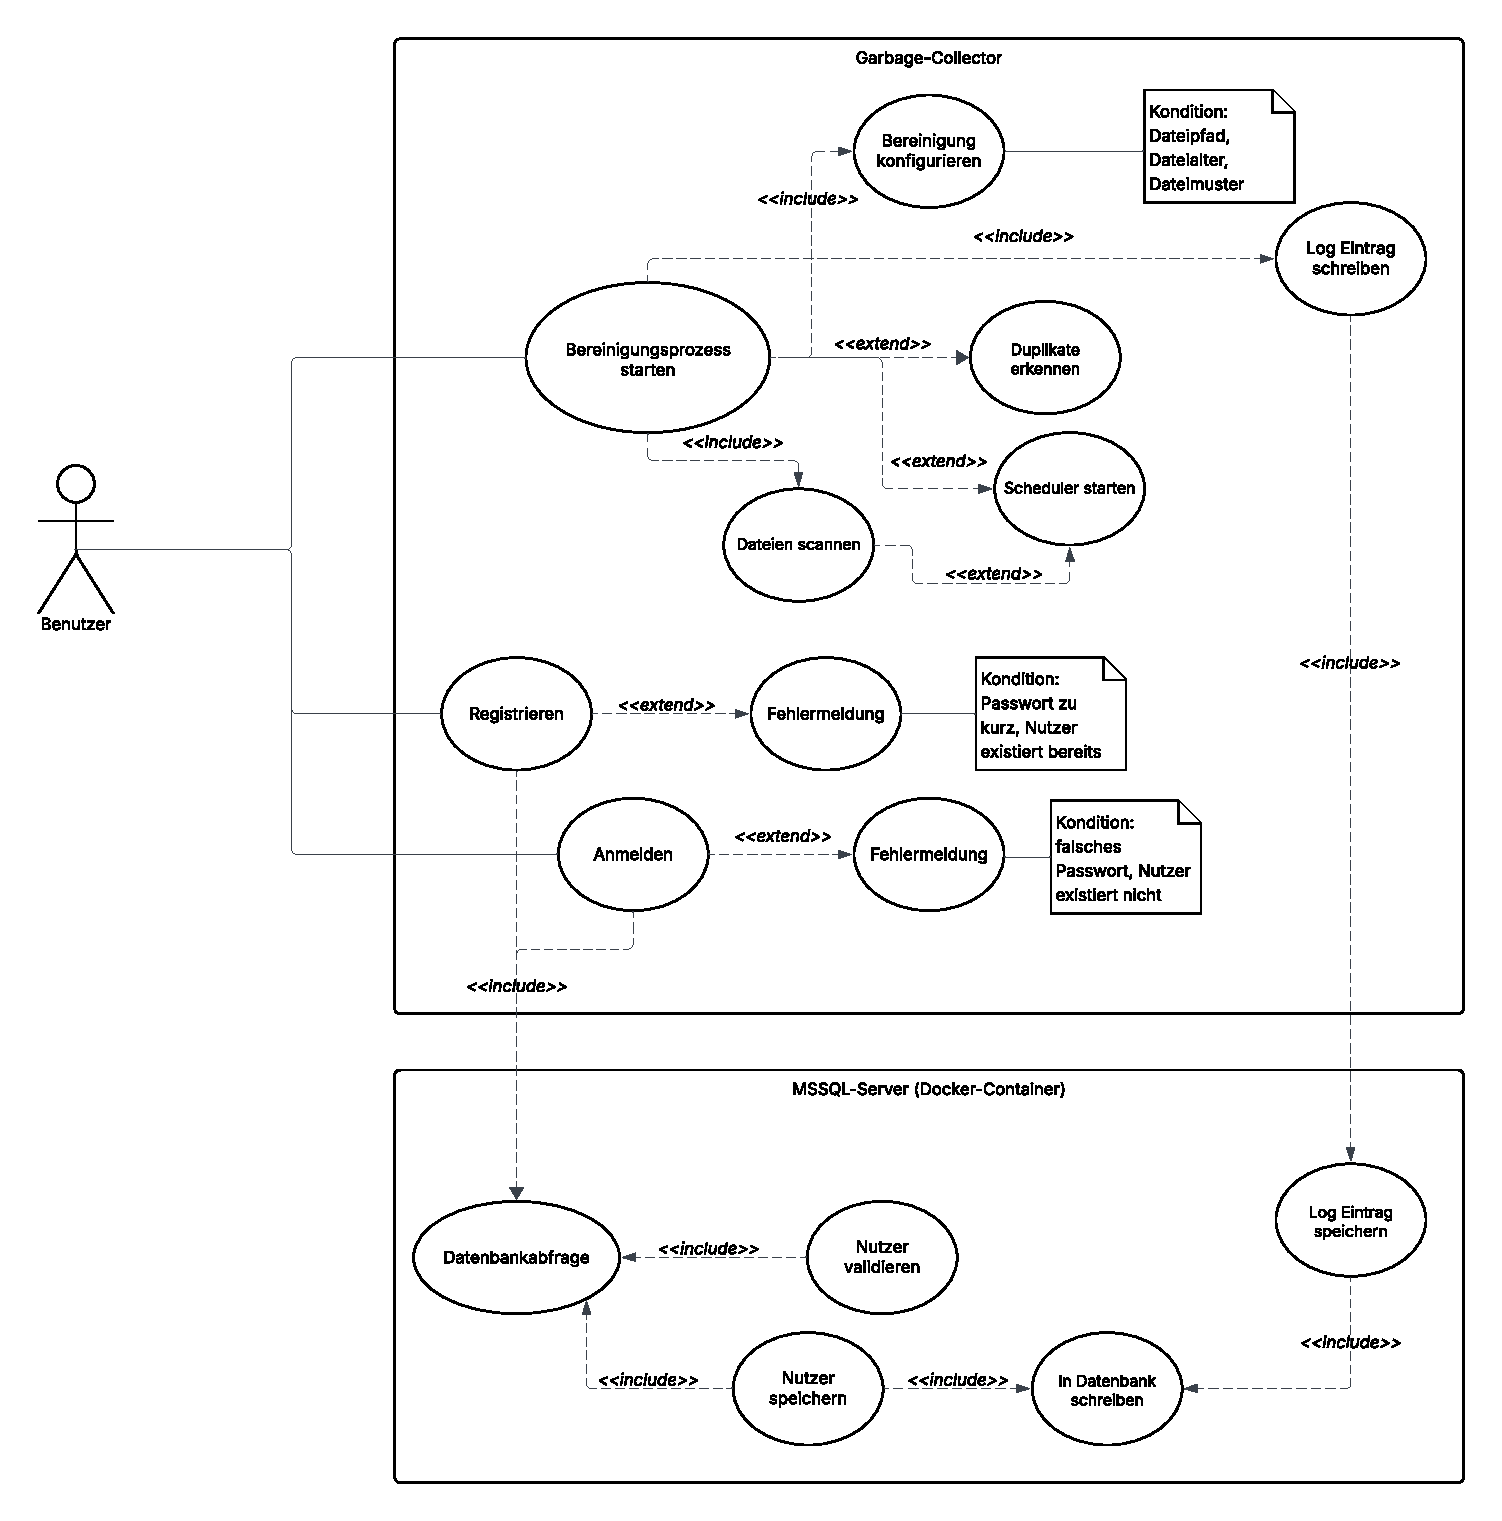
\includegraphics[width=\textwidth]{src/usecase_diagramm.pdf} 
    \caption{Use-Case-Diagramm des Garbage-Collection-Tools}
\end{figure}

\vspace{-0.5em}
\begin{footnotesize}
\textit{Hinweis: Das dargestellte Use-Case-Diagramm fokussiert sich auf die zentralen Anwendungsfälle des Garbage-Collection-Tools. Zusätzliche Funktionen wie Passwortänderung, Adminbereich oder weitere erweiterte Funktionen wurden aus Gründen der Übersichtlichkeit nicht aufgenommen und werden im weiteren Verlauf detaillierter beschrieben.}
\end{footnotesize}


\label{sec:usecases}

\subsubsection*{Use Case: Benutzer registrieren}
\begin{tabular}{|p{5cm}|p{10cm}|}
\hline
\textbf{Kurzbeschreibung} & Ein Benutzer erstellt ein neues Benutzerkonto im Garbage-Collector-Tool. \\
\hline
\textbf{Voraussetzung} & Der Benutzer ist noch nicht registriert. \\
\hline
\textbf{Nachbedingung} & Der Benutzer ist erfolgreich in der Datenbank gespeichert und kann sich künftig anmelden. \\
\hline
\textbf{Fehlersituation} & Das eingegebene Passwort ist zu kurz oder der Benutzername existiert bereits. \\
\hline
\textbf{Systemzustand im Fehlerfall} & Der Benutzer wird nicht registriert, eine Fehlermeldung wird angezeigt. \\
\hline
\textbf{Akteure} & Benutzer \\
\hline
\textbf{Trigger} & Der Benutzer klickt auf „Registrieren“ und füllt das Formular aus. \\
\hline
\textbf{Standardablauf} &
\begin{enumerate}
    \item Der Benutzer öffnet das Garbage-Collector-Tool.
    \item Der Benutzer klickt auf „Registrieren“.
    \item Das Tool prüft die Eingaben (z.\,B. Passwortlänge, eindeutiger Benutzername).
    \item Die Daten werden über eine Datenbankabfrage gespeichert.
    \item Der Benutzer erhält eine Bestätigung zur erfolgreichen Registrierung.
\end{enumerate}
\\
\hline
\textbf{Alternativabläufe} &
\begin{itemize}
    \item Das Passwort ist zu kurz.
    \item Der Benutzername ist bereits vergeben.
    \item Eine Fehlermeldung wird angezeigt und der Benutzer muss die Eingaben korrigieren.
\end{itemize}
\\
\hline
\end{tabular}


\subsubsection*{Use Case: Benutzer anmelden}
\begin{tabular}{|p{5cm}|p{10cm}|}
\hline
\textbf{Kurzbeschreibung} & Ein Benutzer meldet sich mit gültigen Zugangsdaten am System an. \\
\hline
\textbf{Voraussetzung} & Der Benutzer ist registriert und besitzt gültige Zugangsdaten. \\
\hline
\textbf{Nachbedingung} & Der Benutzer ist authentifiziert und erhält Zugriff auf die Funktionen der Software. \\
\hline
\textbf{Fehlersituation} & Das Passwort ist falsch oder der Benutzer existiert nicht. \\
\hline
\textbf{Systemzustand im Fehlerfall} & Keine Anmeldung, Zugriff wird verweigert, Fehlermeldung wird angezeigt. \\
\hline
\textbf{Akteure} & Benutzer \\
\hline
\textbf{Trigger} & Der Benutzer klickt auf „Anmelden“ und gibt Zugangsdaten ein. \\
\hline
\textbf{Standardablauf} &
\begin{enumerate}
    \item Der Benutzer öffnet das Tool und wählt „Anmelden“.
    \item Die Zugangsdaten werden über eine Datenbankabfrage geprüft.
    \item Die Anmeldung wird bestätigt.
    \item Der Benutzer hat Zugriff auf die Funktionen.
\end{enumerate}
\\
\hline
\textbf{Alternativabläufe} &
\begin{itemize}
    \item Falsches Passwort oder nicht existierender Benutzer.
    \item Fehlermeldung wird angezeigt, keine Anmeldung erfolgt.
\end{itemize}
\\
\hline
\end{tabular}

\vspace{1cm}

\subsubsection*{Use Case: Duplikate erkennen}
\begin{tabular}{|p{5cm}|p{10cm}|}
\hline
\textbf{Kurzbeschreibung} & Das Tool durchsucht die zu bereinigenden Dateien nach Duplikaten. \\
\hline
\textbf{Voraussetzung} & Die Bereinigung wurde gestartet. \\
\hline
\textbf{Nachbedingung} & Gefundene Duplikate werden zur weiteren Bearbeitung markiert oder entfernt. \\
\hline
\textbf{Fehlersituation} & Das System kann keine Duplikate erkennen (z.\,B. durch falsche Pfadangabe). \\
\hline
\textbf{Systemzustand im Fehlerfall} & Es werden keine Duplikate entfernt. \\
\hline
\textbf{Akteure} & Benutzer \\
\hline
\textbf{Trigger} & Der Benutzer startet die Bereinigung, das Duplikat-Erkennungsmodul wird automatisch aktiviert. \\
\hline
\textbf{Standardablauf} &
\begin{enumerate}
    \item Der Benutzer startet die Bereinigung.
    \item Das System durchsucht die angegebenen Verzeichnisse.
    \item Duplikate werden erkannt und entfernt oder dem Benutzer angezeigt.
    \item Ein Log-Eintrag wird erstellt.
\end{enumerate}
\\
\hline
\textbf{Alternativabläufe} &
\begin{itemize}
    \item Keine Duplikate gefunden.
    \item Das Duplikatmodul schlägt fehl, Log wird trotzdem erstellt.
\end{itemize}
\\
\hline
\end{tabular}

\vspace{1cm}

\subsubsection*{Use Case: Scheduler starten}
\begin{tabular}{|p{5cm}|p{10cm}|}
\hline
\textbf{Kurzbeschreibung} & Das Tool aktiviert eine Zeitsteuerung zur automatischen Durchführung von Bereinigungen. \\
\hline
\textbf{Voraussetzung} & Der Benutzer hat eine Konfiguration und den Zeitintervall festgelegt. \\
\hline
\textbf{Nachbedingung} & Der Scheduler ist aktiv und führt Bereinigungen gemäß Plan durch. \\
\hline
\textbf{Fehlersituation} & Es wurde kein oder ein falscher Pfad angegeben \\
\hline
\textbf{Systemzustand im Fehlerfall} & Keine automatische Bereinigung erfolgt. \\
\hline
\textbf{Akteure} & Benutzer \\
\hline
\textbf{Trigger} & Der Benutzer speichert eine Zeitsteuerung im Tool und startet den Scheduler. \\
\hline
\textbf{Standardablauf} &
\begin{enumerate}
    \item Der Benutzer öffnet die Einstellungen.
    \item Er konfiguriert einen automatischen Zeitplan.
    \item Der Benutzer aktiviert den internen Scheduler.
    \item Die geplanten Bereinigungen werden zum festgelegten Zeitintervall durchgeführt.
\end{enumerate}
\\
\hline
\textbf{Alternativabläufe} &
\begin{itemize}
    \item Ungültige Zeitangabe verhindert die Aktivierung.
    \item Fehlerhafte Konfiguration wird vom Tool gemeldet.
\end{itemize}
\\
\hline
\end{tabular}

\vspace{1cm}

\subsubsection*{Use Case: Log-Eintrag schreiben und speichern}
\begin{tabular}{|p{5cm}|p{10cm}|}
\hline
\textbf{Kurzbeschreibung} & Bei jedem Bereinigungsvorgang wird ein Log-Eintrag erstellt und in der Datenbank gespeichert. \\
\hline
\textbf{Voraussetzung} & Eine der drei Bereinigungstypen (Standard, Duplikate, Junk-Dateien)  oder Scheduler wurden ausgeführt \\
\hline
\textbf{Nachbedingung} & Ein entsprechender Eintrag befindet sich in der Log-Datenbank und steht zum Download bereit \\
\hline
\textbf{Fehlersituation} & Die Verbindung zur Datenbank ist unterbrochen oder Schreibrechte fehlen. \\
\hline
\textbf{Systemzustand im Fehlerfall} & Kein Eintrag in der Datenbank oder keine Verbindung \\
\hline
\textbf{Akteure} & (Internes Systemverhalten, ausgelöst durch Benutzeraktionen) \\
\hline
\textbf{Trigger} & Es wurde eine Bereinigung durch den Benutzer oder den Scheduler durchgeführt \\
\hline
\textbf{Standardablauf} &
\begin{enumerate}
    \item Eine Benutzeraktion (z.\,B. Start Bereinigung) wird ausgeführt.
    \item Das System erzeugt einen Log-Eintrag.
    \item Der Log-Eintrag wird an den MSSQL-Server weitergeleitet.
    \item Der Eintrag wird dauerhaft gespeichert.
\end{enumerate}
\\
\hline
\textbf{Alternativabläufe} &
\begin{itemize}
    \item Verbindung zur Datenbank schlägt fehl.
\end{itemize}
\\
\hline
\end{tabular}
\subsection{Projektplan}
\begin{figure}[H]
    \centering
    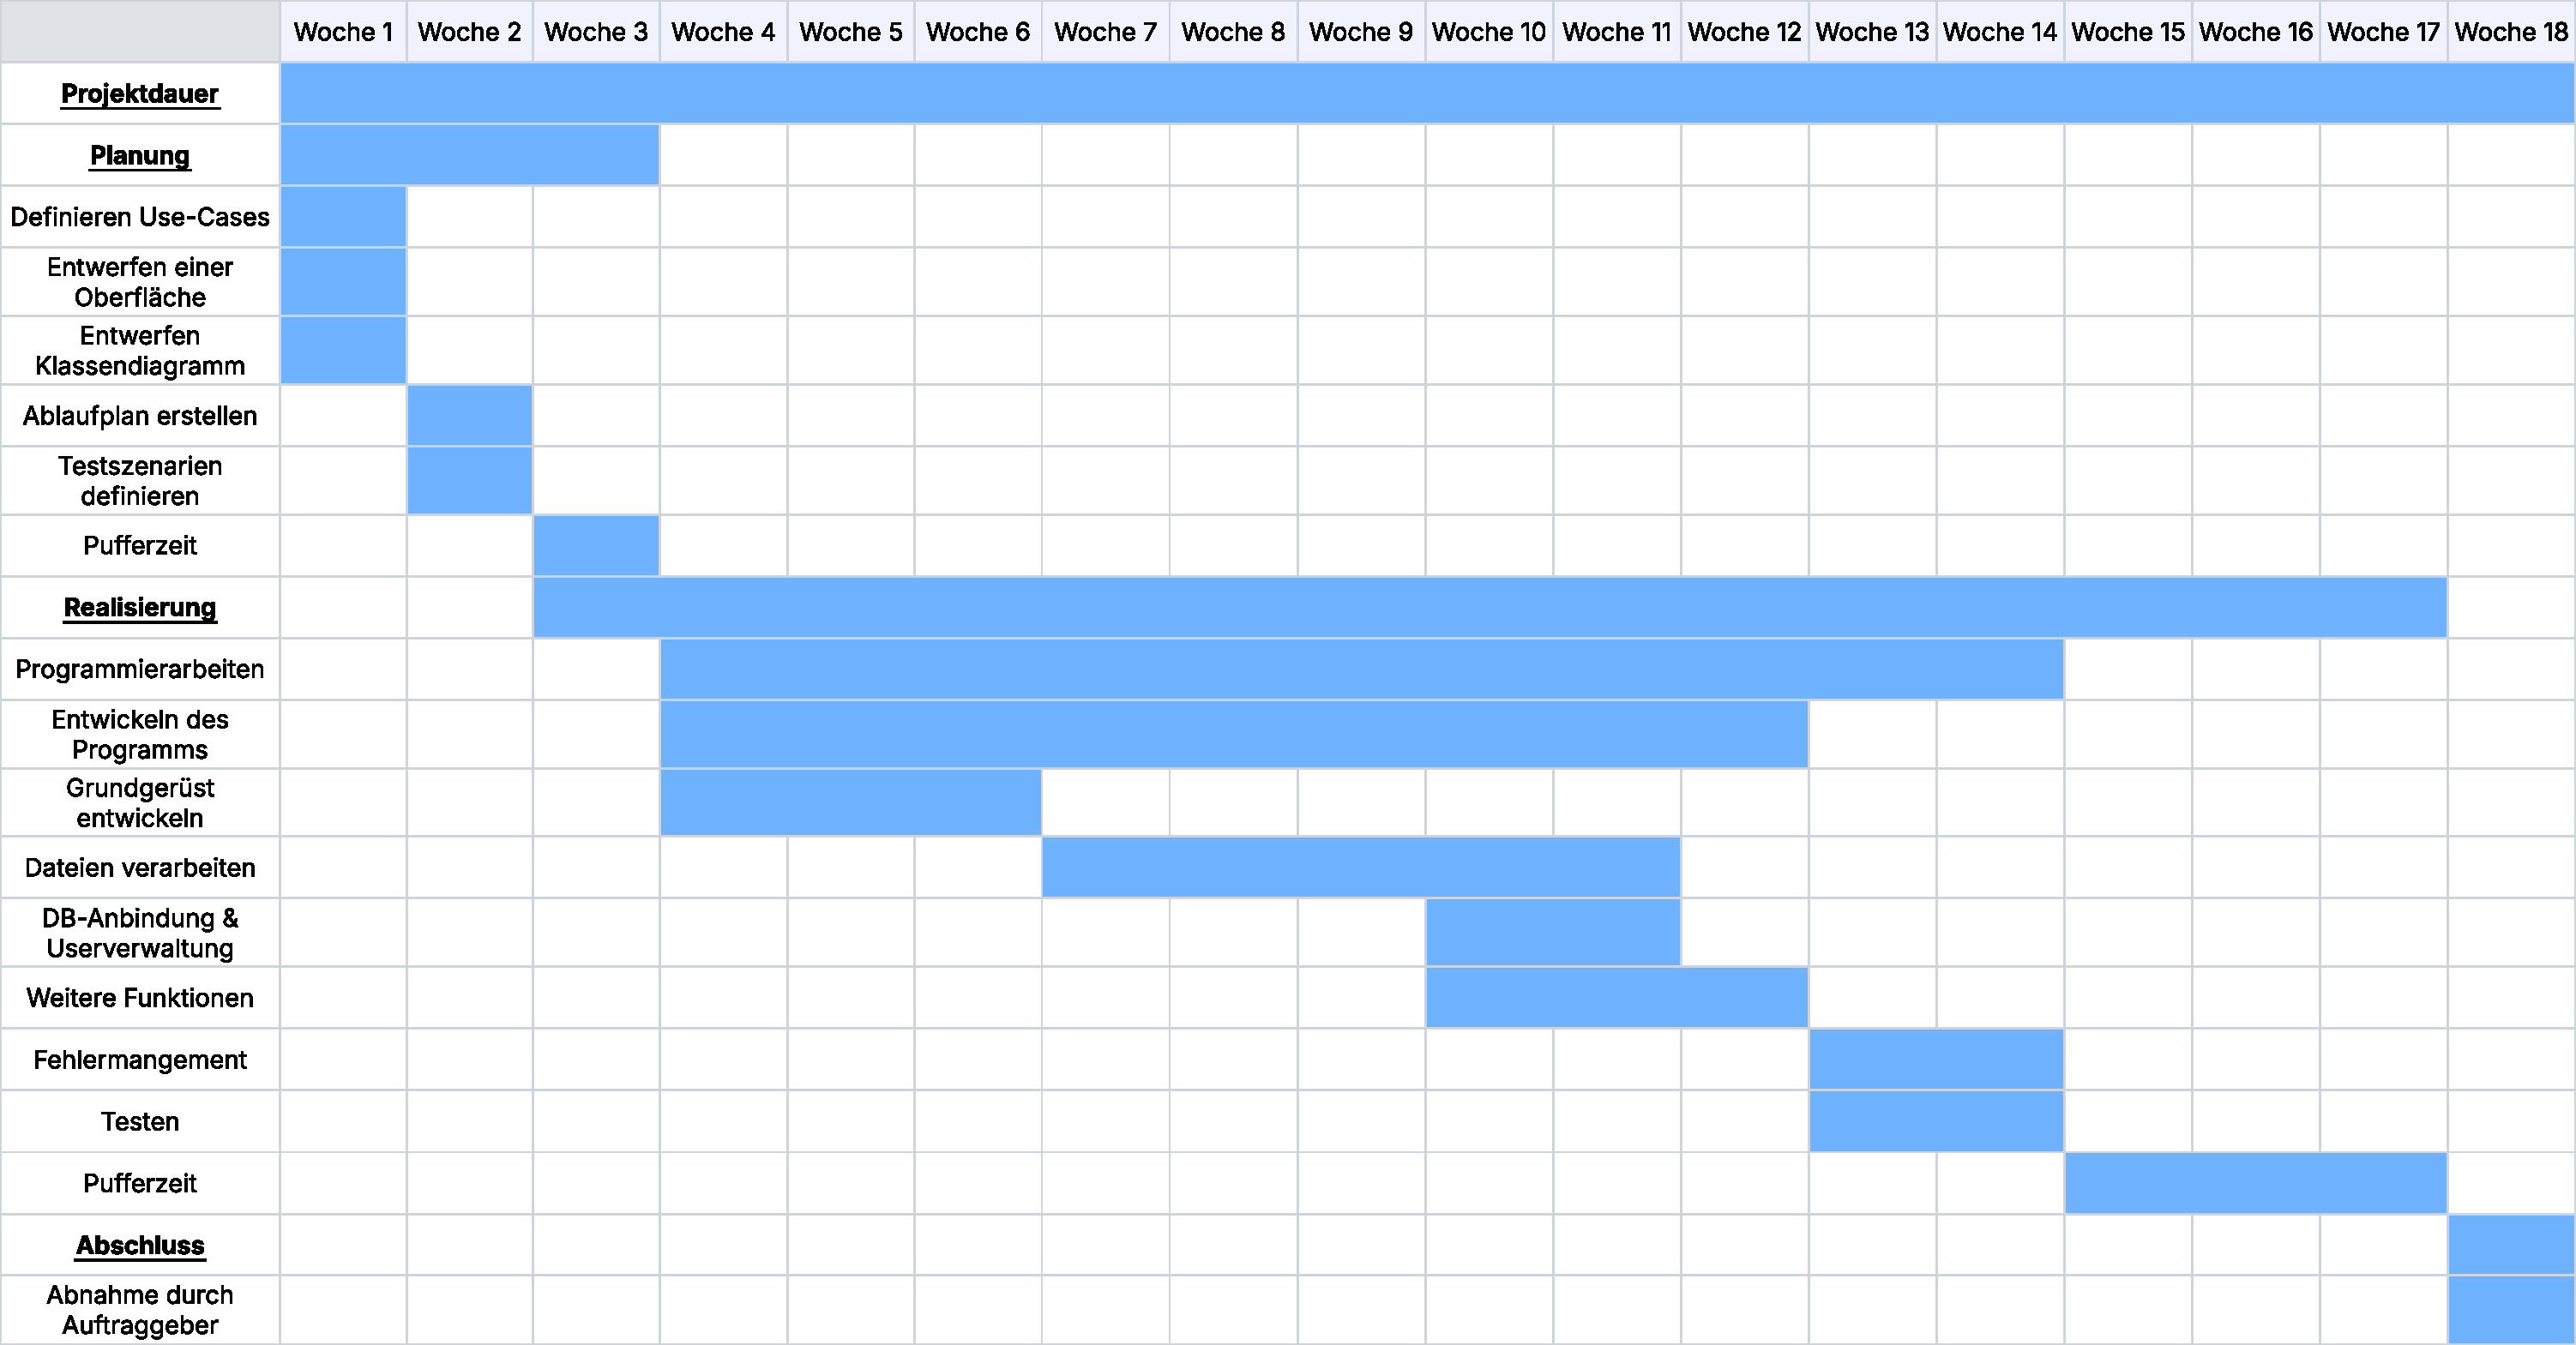
\includegraphics[width=\textwidth]{src/gantt_diagramm.pdf} 
    \caption{Projektplan als Gantt-Diagramm}
\end{figure}
\subsection{Produktumgebung}


Für die Entwicklung und den Einsatz des Garbage-Collection-Tools wurde folgende technische Produktumgebung verwendet:

\begin{itemize} \item \textbf{Programmiersprache:}
Die Anwendung wurde in \textbf{C\#} entwickelt, da die Sprache eine umfangreiche Unterstützung für Windows-basierte Desktop-Anwendungen bietet und eine moderne objektorientierte Programmierung ermöglicht.

\item \textbf{UI-Design:}
Das Layout und die Benutzeroberfläche wurden zunächst mit \textbf{Figma} entworfen. Dieses Tool ermöglicht eine effiziente Erstellung von Prototypen und UI-Komponenten, die anschließend in die WPF-Oberfläche übertragen wurden.

\item \textbf{Entwicklungsumgebung:}
Zur Umsetzung kam \textbf{Visual Studio} zum Einsatz. Die integrierte Entwicklungsumgebung (IDE) bietet umfassende Werkzeuge für C\#-Projekte, Debugging, Versionskontrolle und Benutzeroberflächendesign.

\item \textbf{Datenbanken:}
Für die persistente Speicherung von Konfigurationsdaten, Benutzerinformationen und Bereinigungsprotokollen wird ein \textbf{SQL Server} verwendet. Dieser wird in einem Docker-Container unter Linux betrieben und ist über das Netzwerk angebunden.

\item \textbf{Betriebssysteme:}
Die Anwendung ist kompatibel mit \textbf{Windows 10} und \textbf{Windows 11}. Die Entwicklung erfolgte unter macOS mithilfe von \textbf{Parallels}, was unter einer Windows 11 VM lief.

 \end{itemize}
\subsection{Skizze des GUI}
\begin{figure}[H]
    \centering
    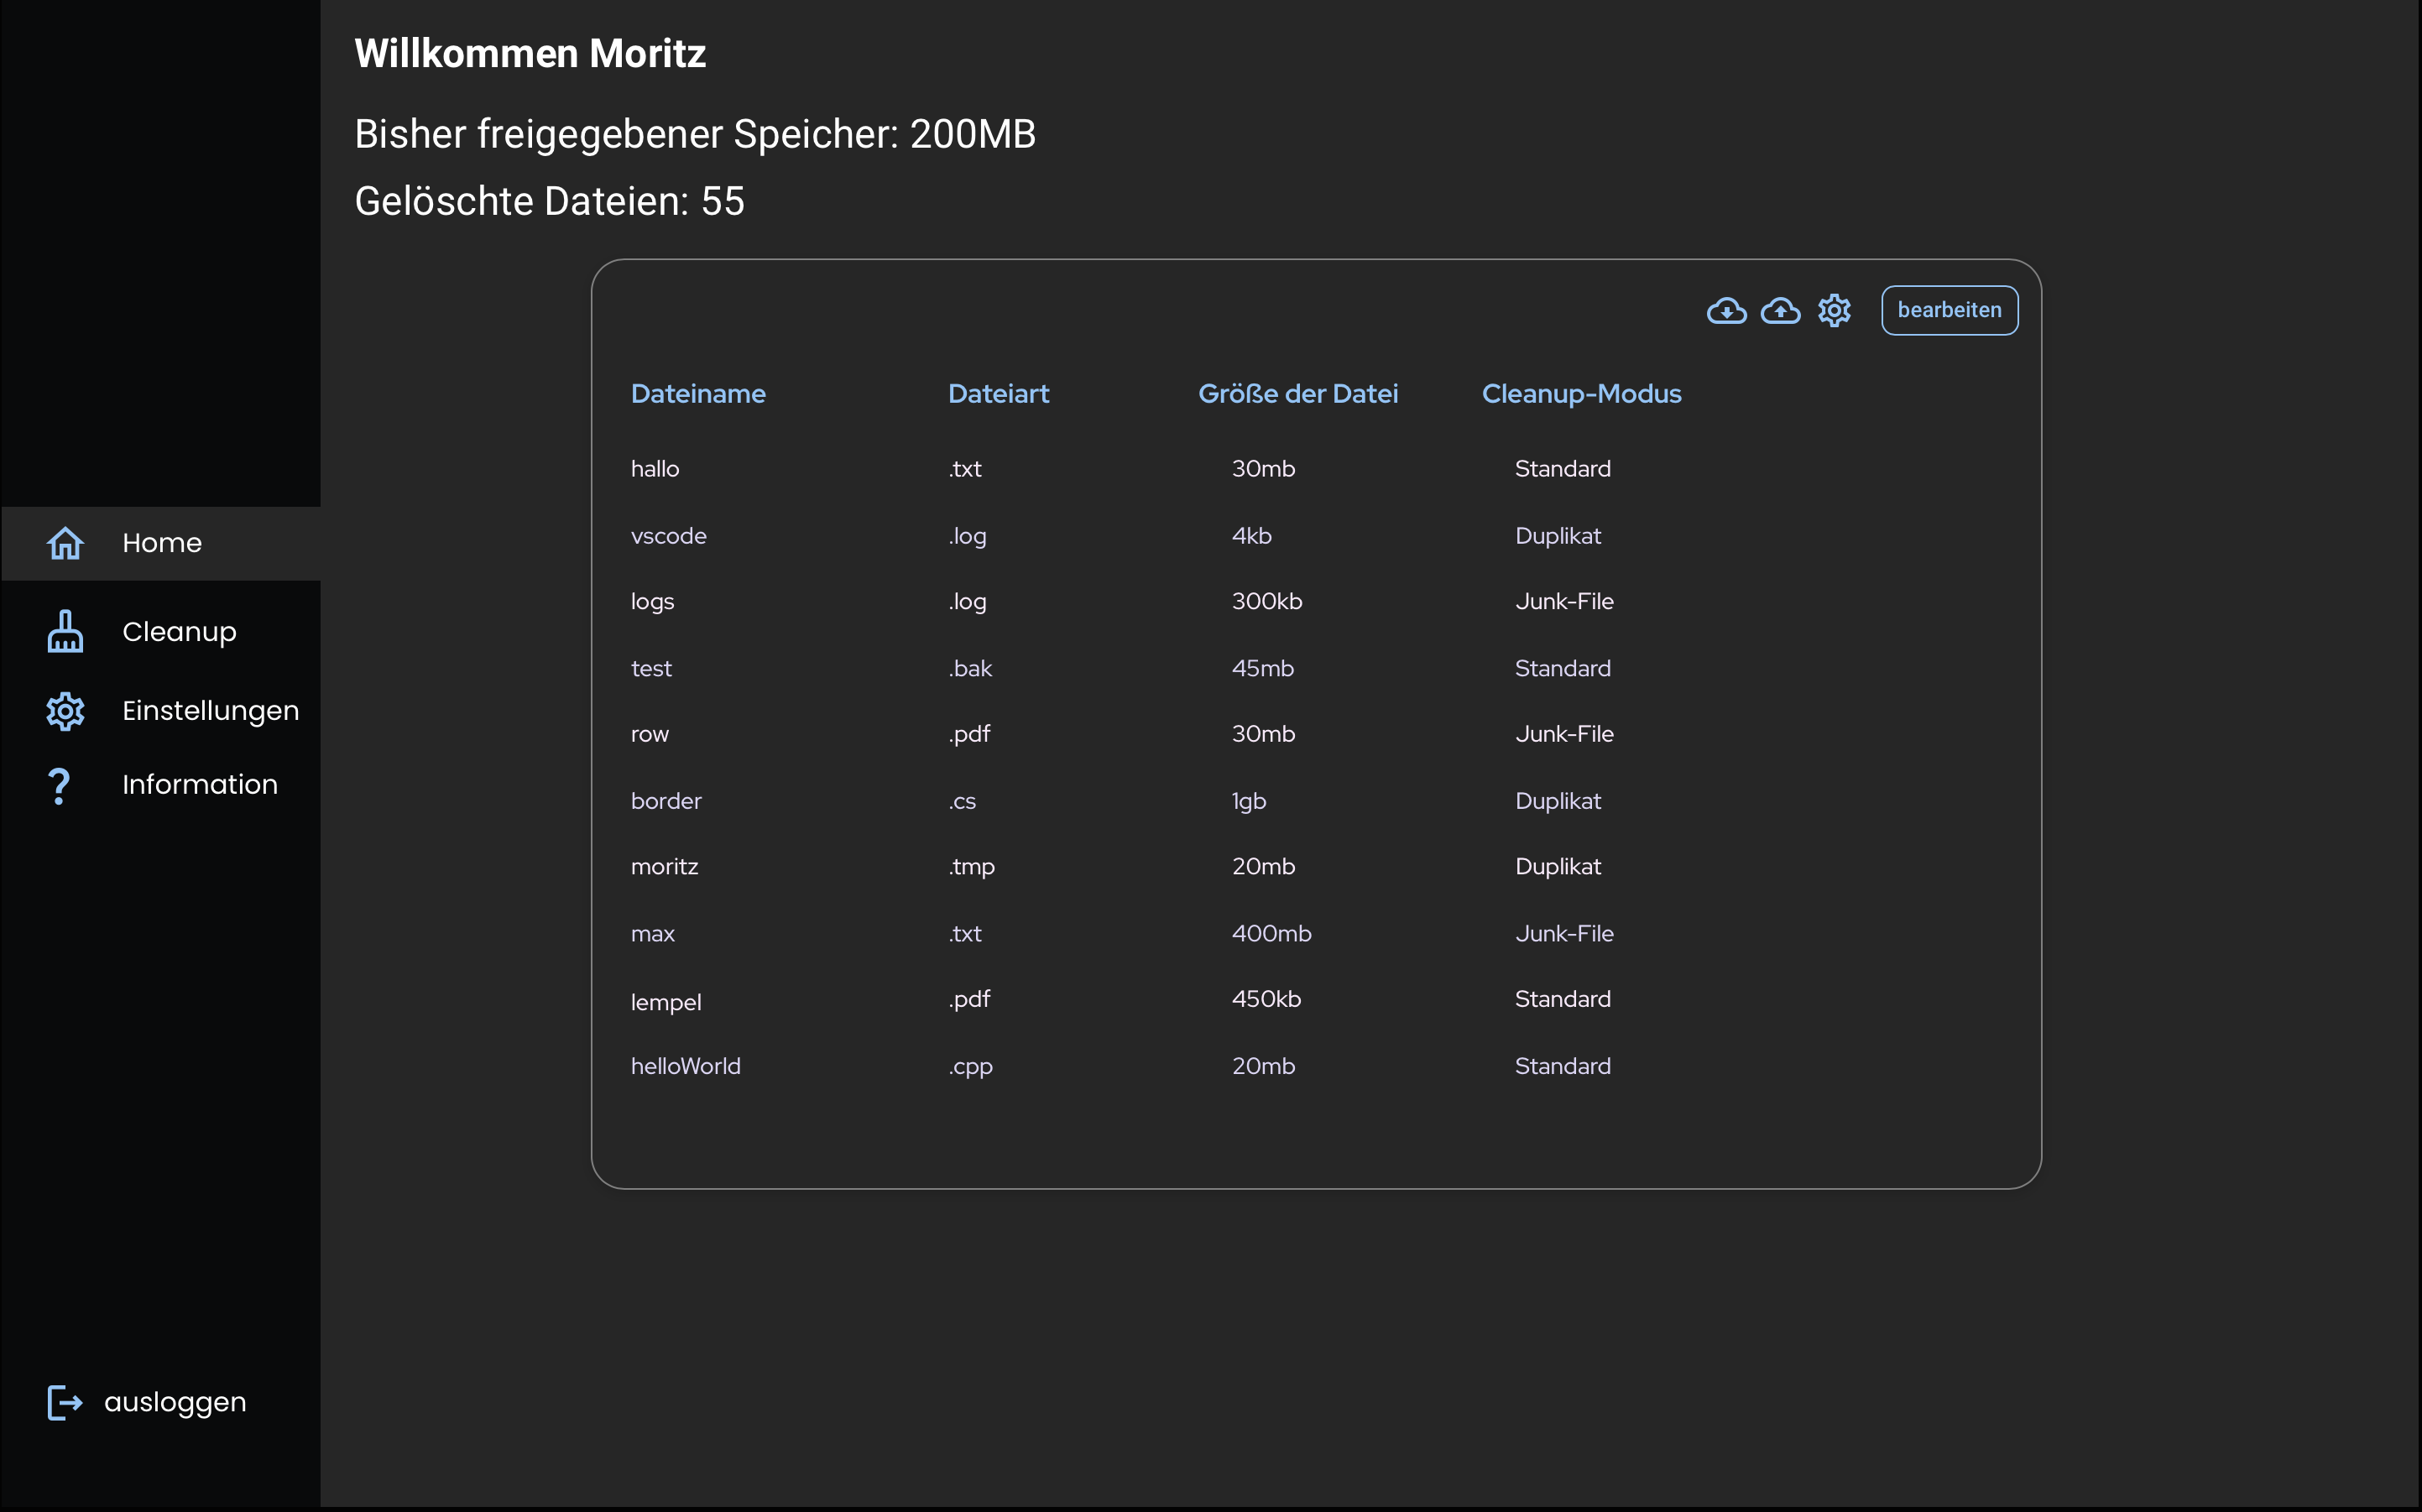
\includegraphics[width=0.95\textwidth]{src/mockup_ui_home.png}
    \caption{GUI-Ansicht: Home}
    \label{fig:gui-home}
\end{figure}

\begin{figure}[H]
    \centering
    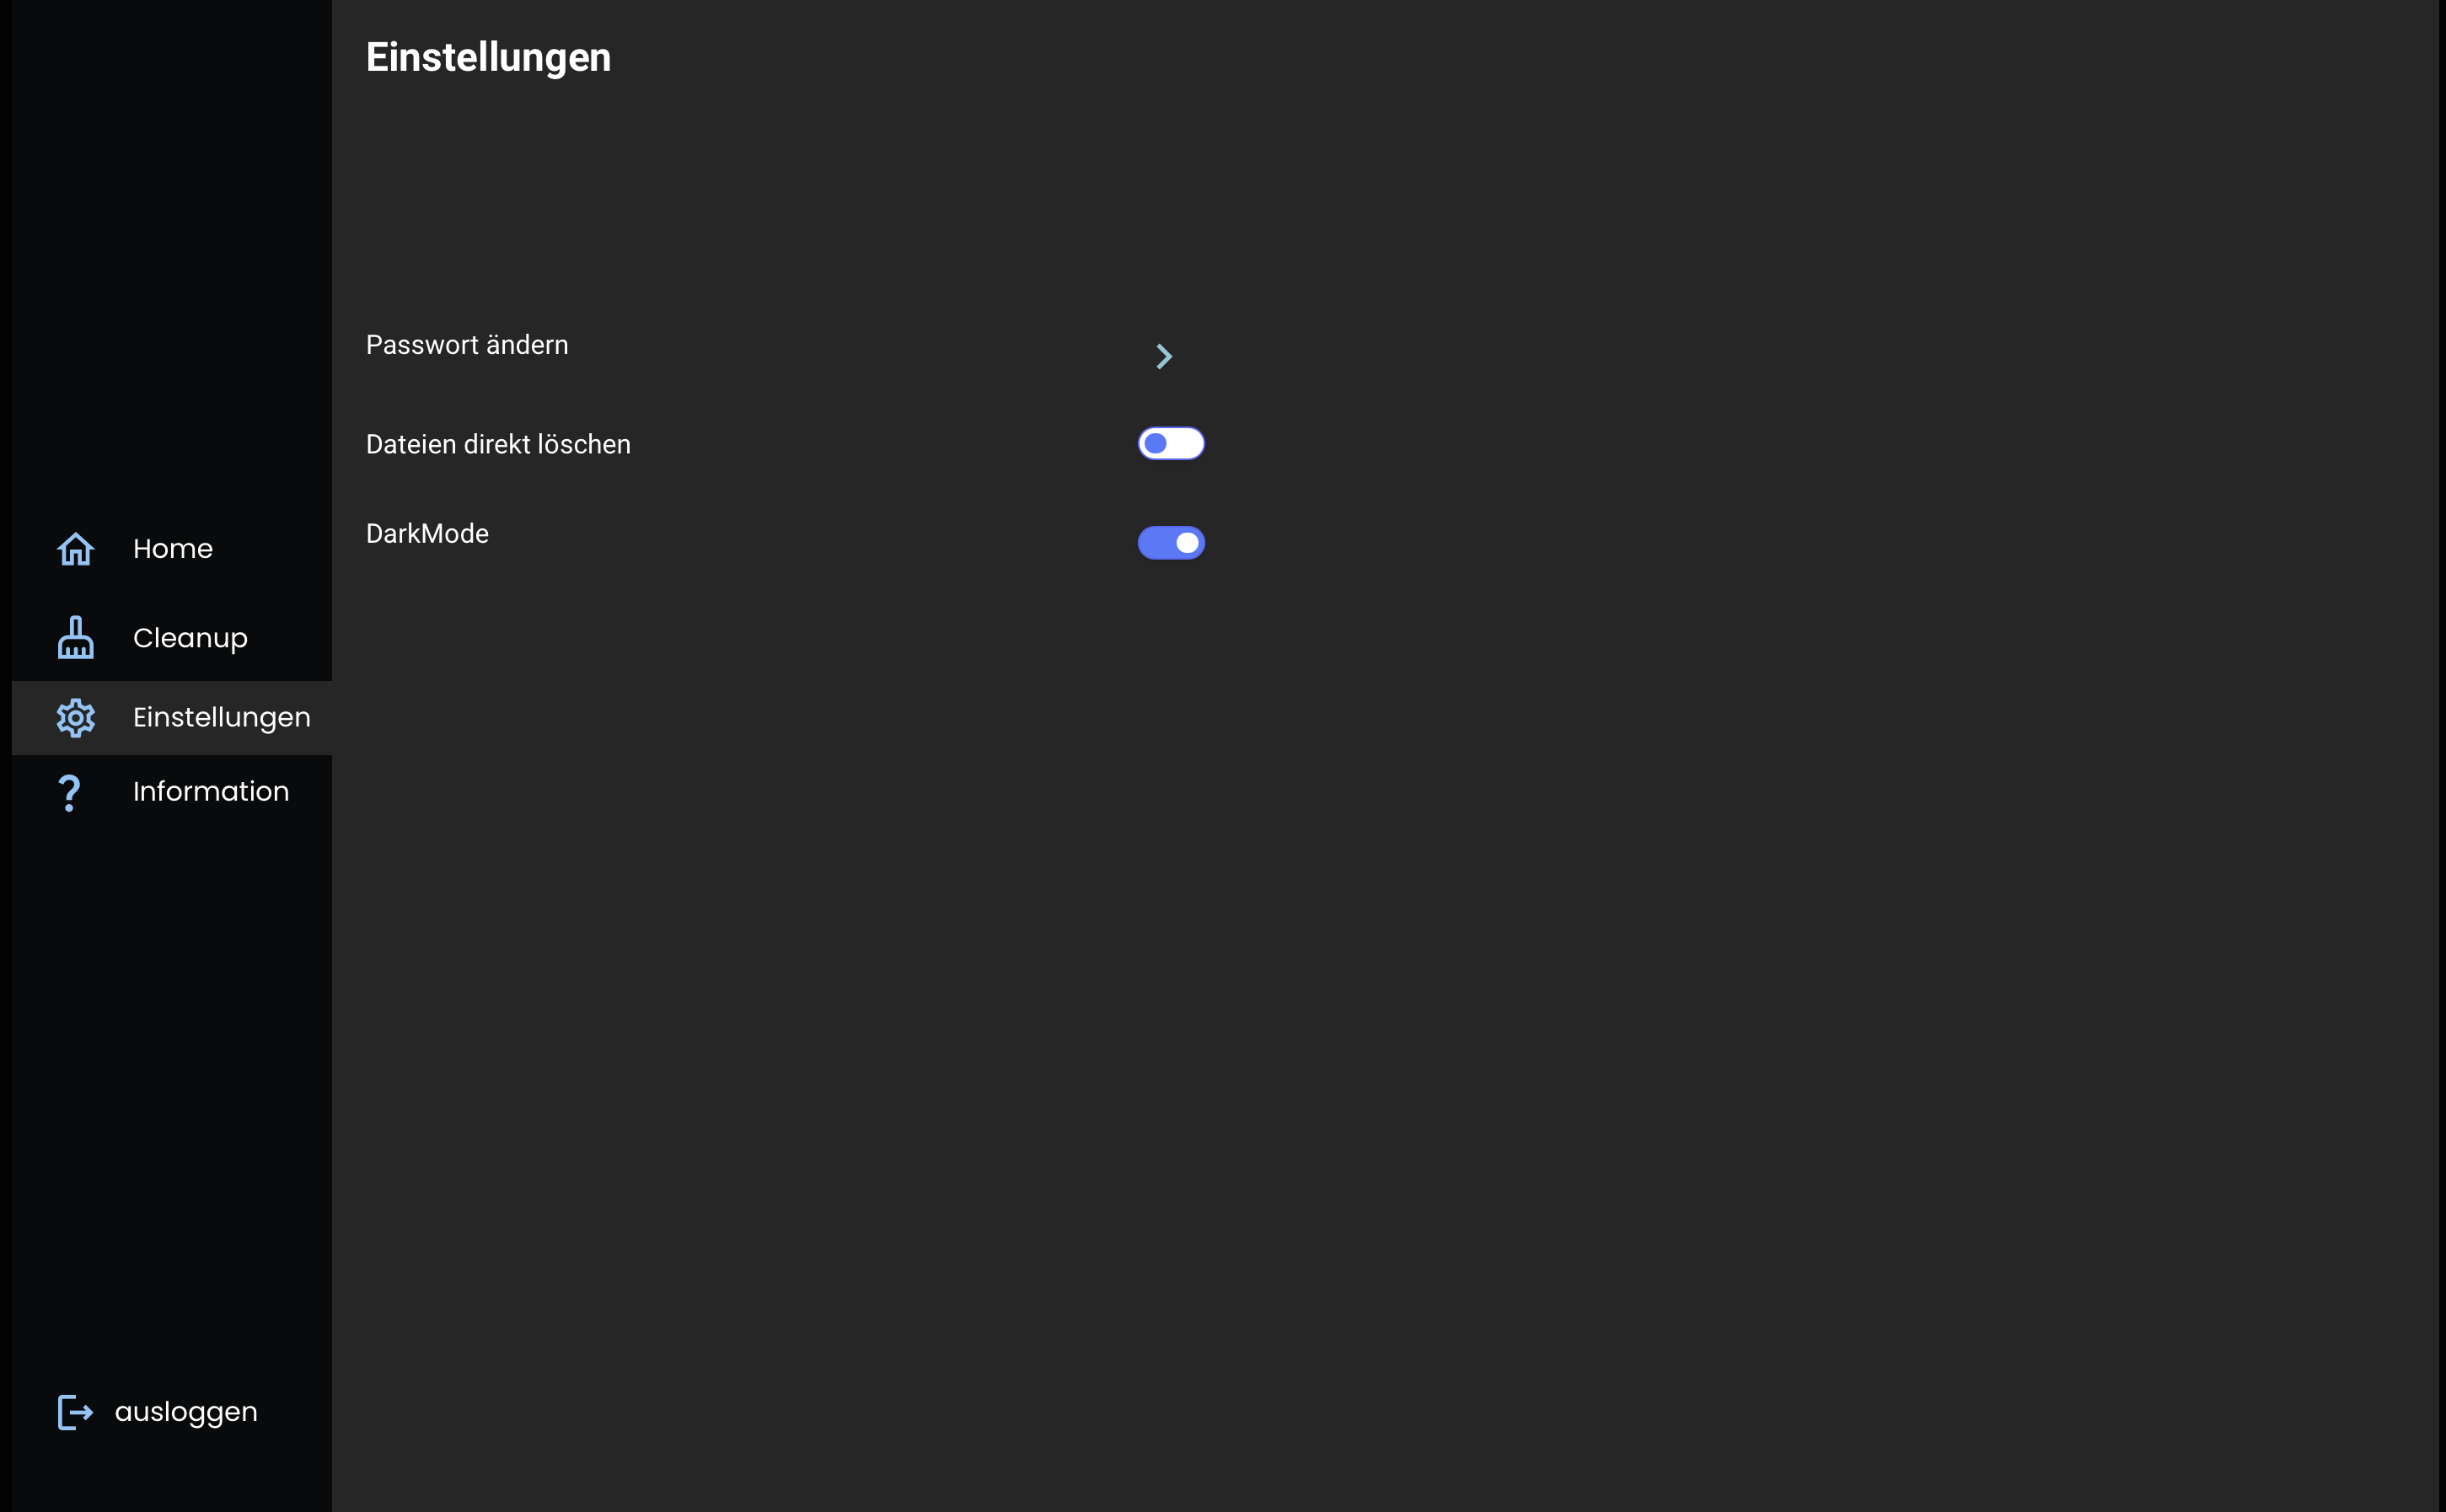
\includegraphics[width=0.95\textwidth]{src/mockup_ui_settings.png}
    \caption{GUI-Ansicht: Einstellungen}
    \label{fig:gui-settings}
\end{figure}

\begin{figure}[H]
    \centering
    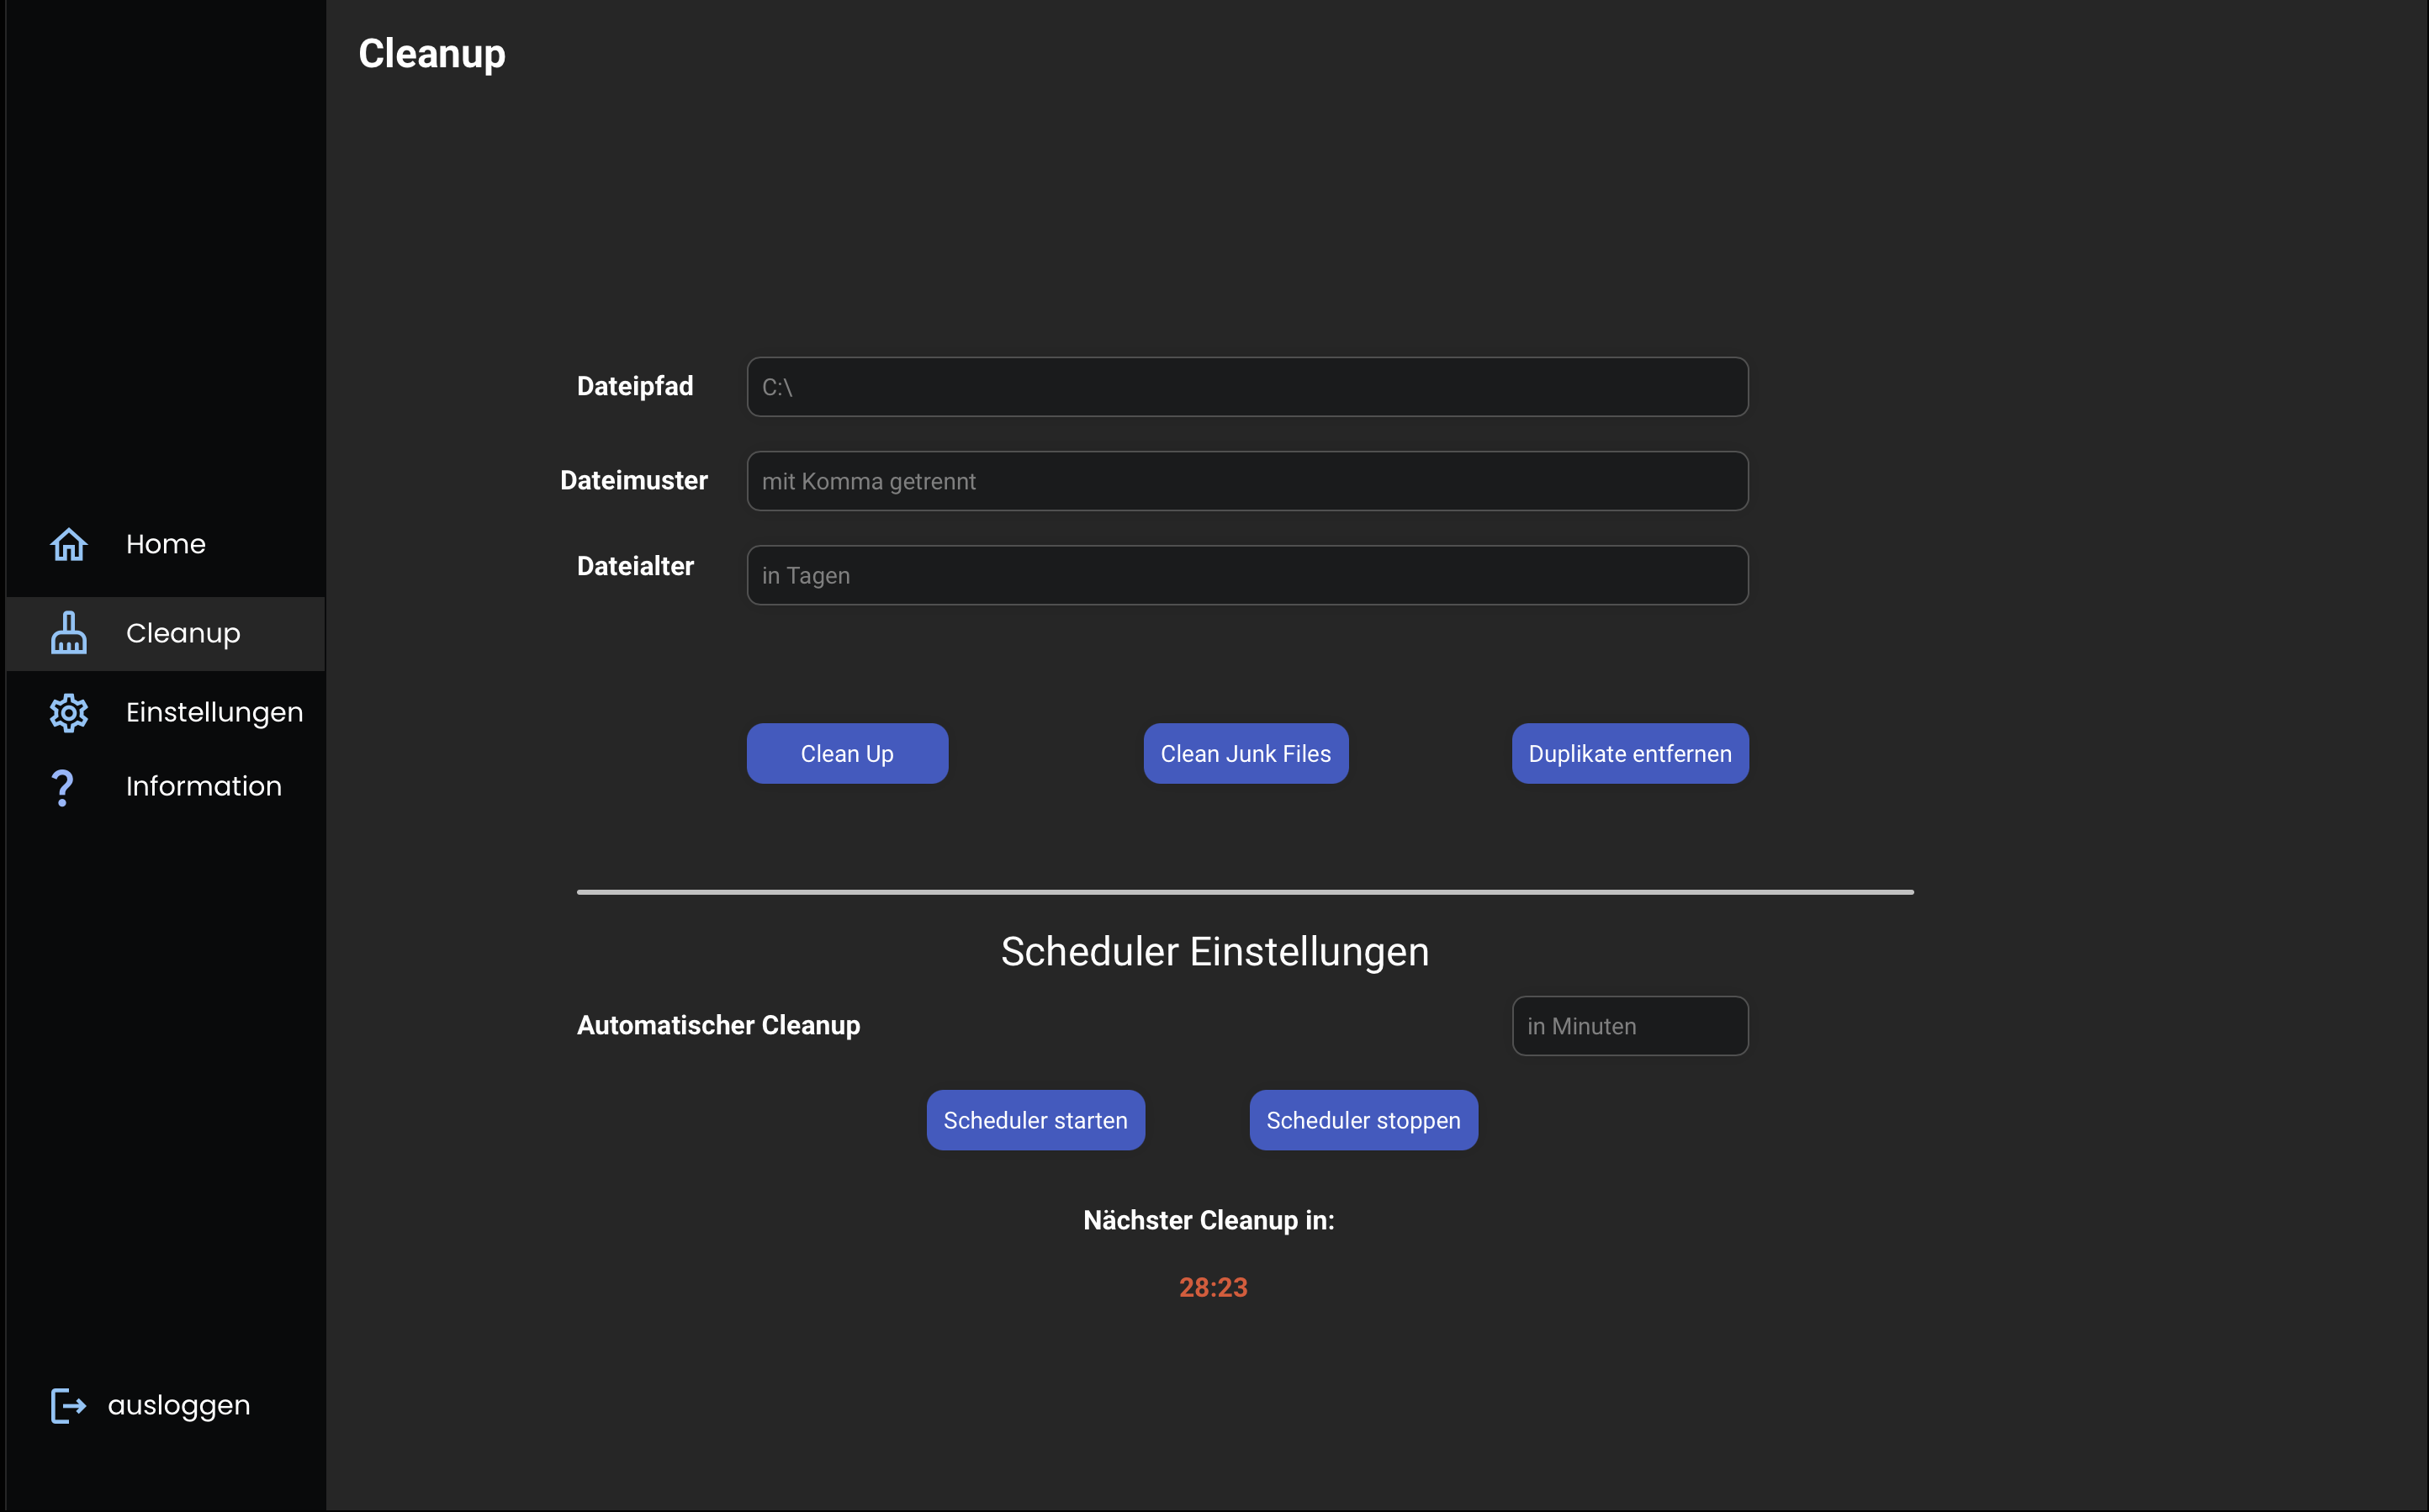
\includegraphics[width=0.95\textwidth]{src/mockup_ui_cleanup.png}
    \caption{GUI-Ansicht: Cleanup}
    \label{fig:gui-cleanup}
\end{figure}

\begin{figure}[H]
    \centering
    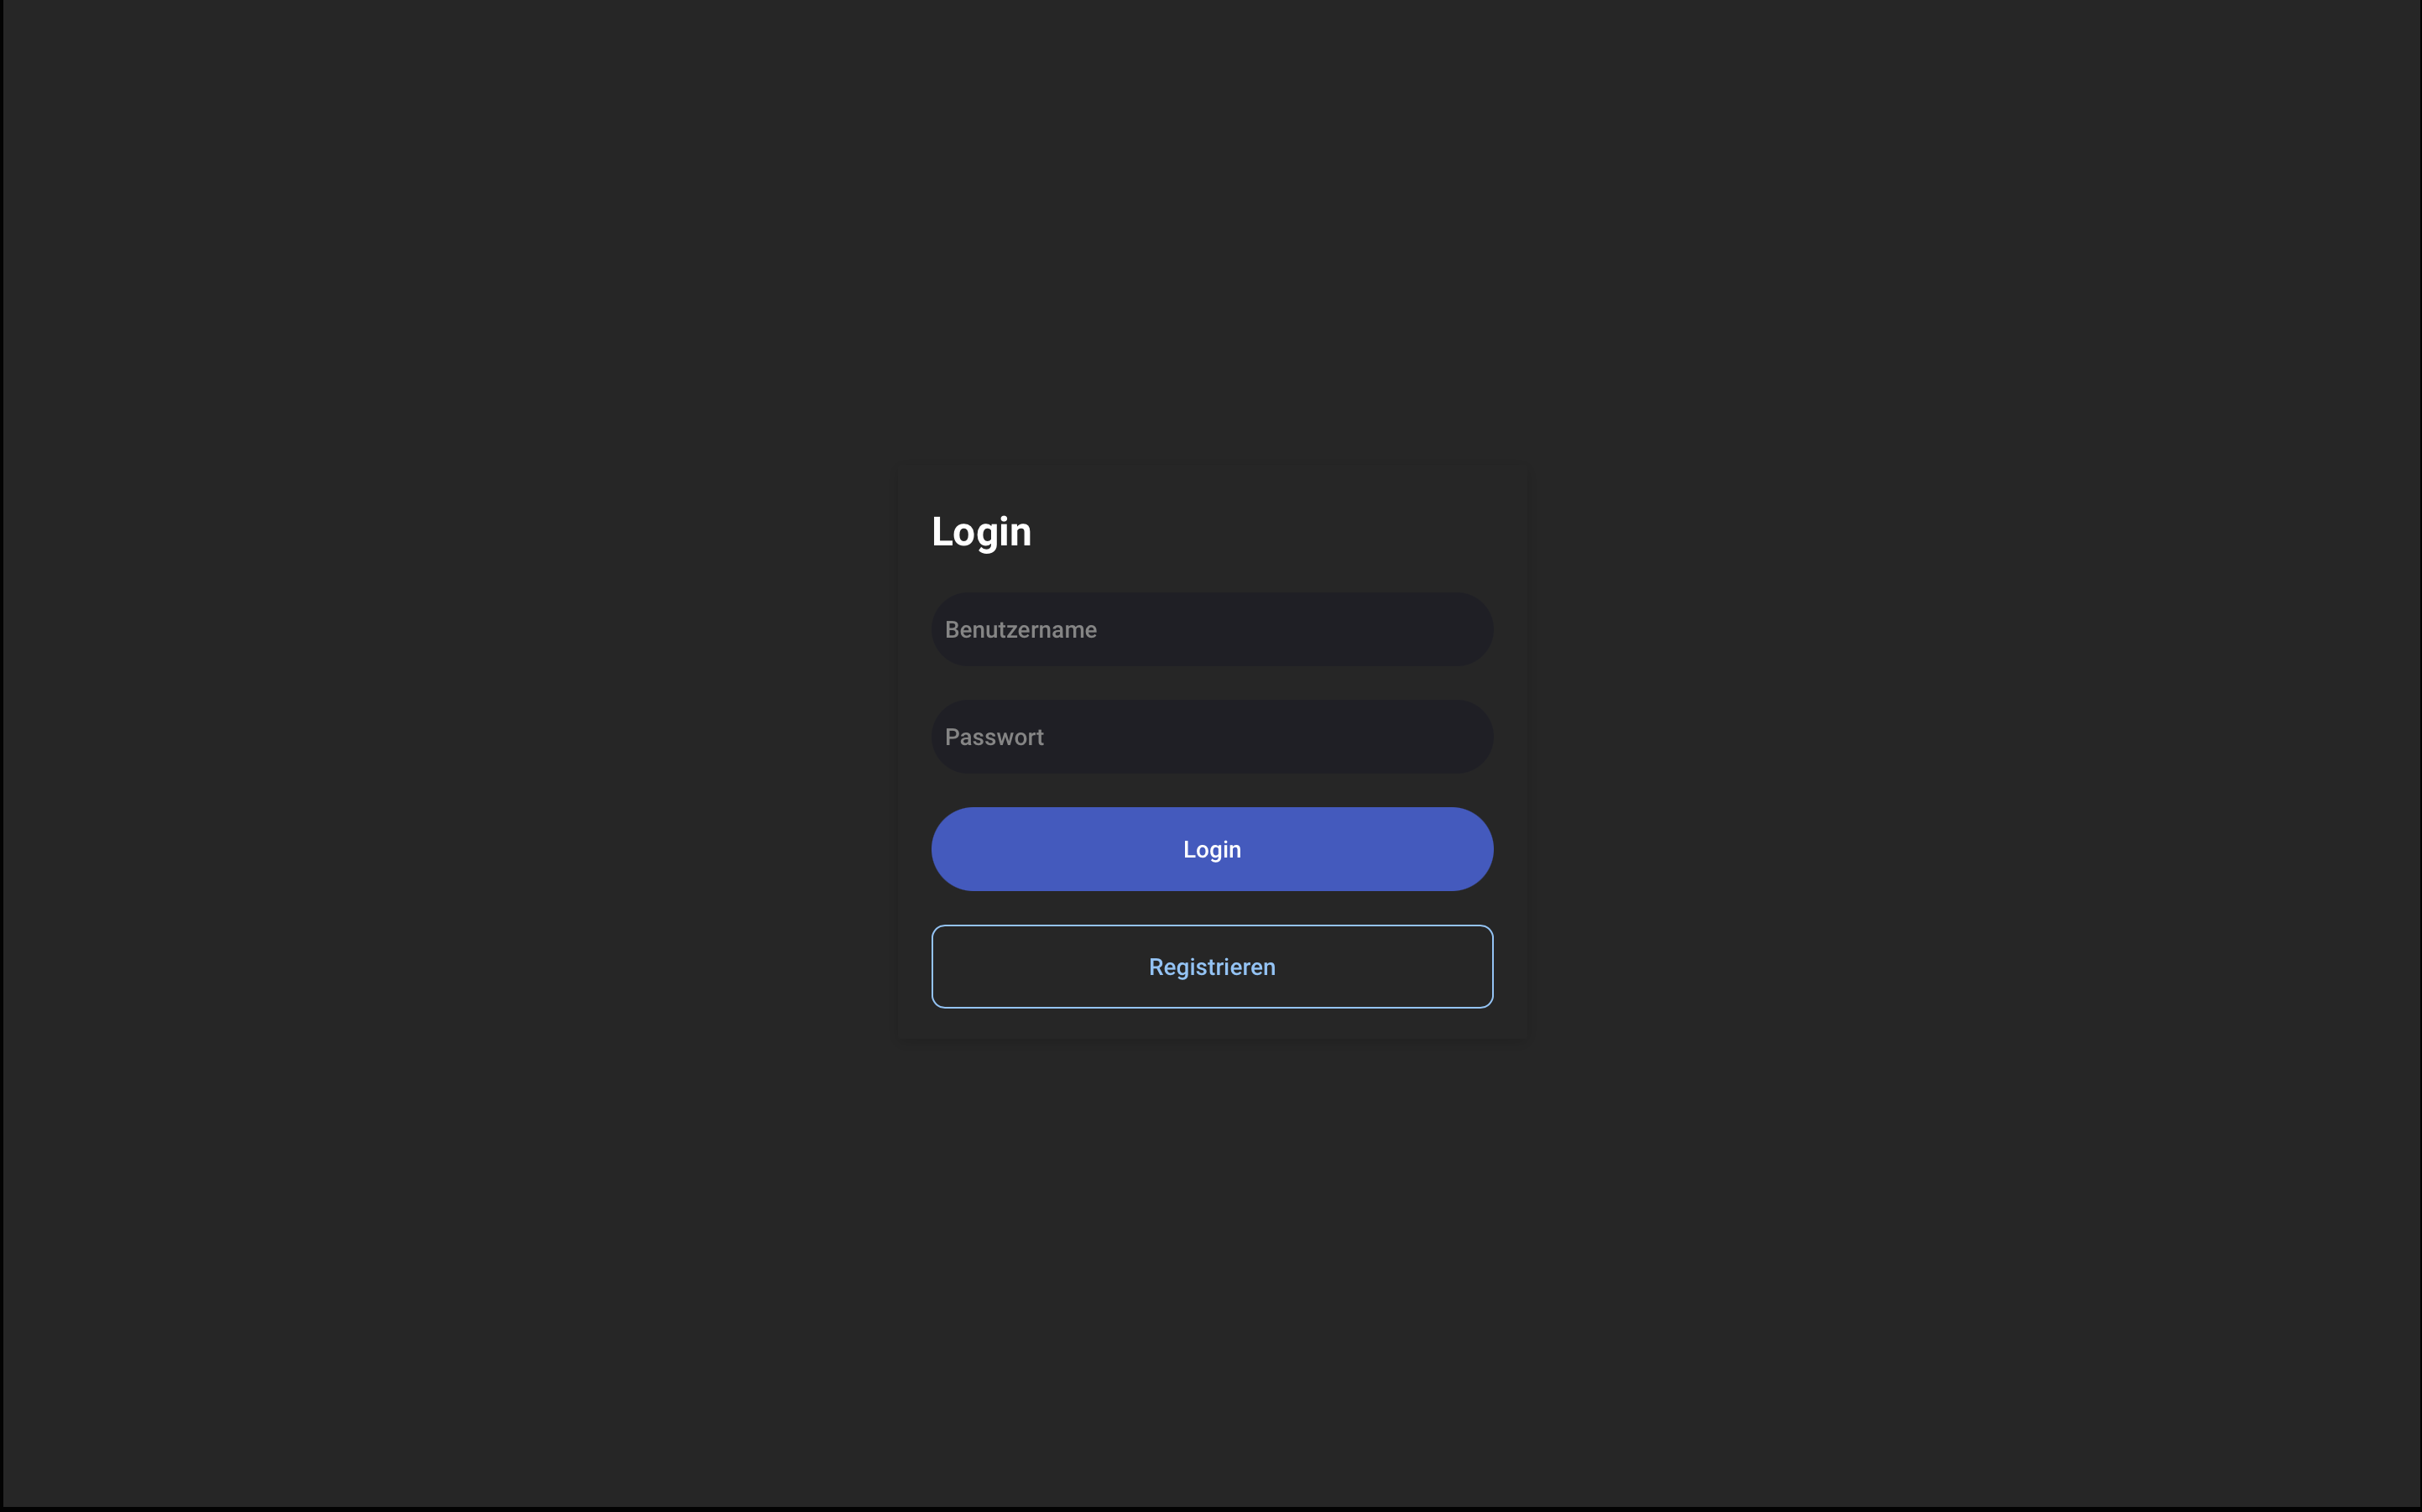
\includegraphics[width=0.95\textwidth]{src/mockup_ui_login.png}
    \caption{GUI-Ansicht: Login}
    \label{fig:gui-login}
\end{figure}

\subsection{DB-Entwurf}



\begin{figure}[H]
    \centering
    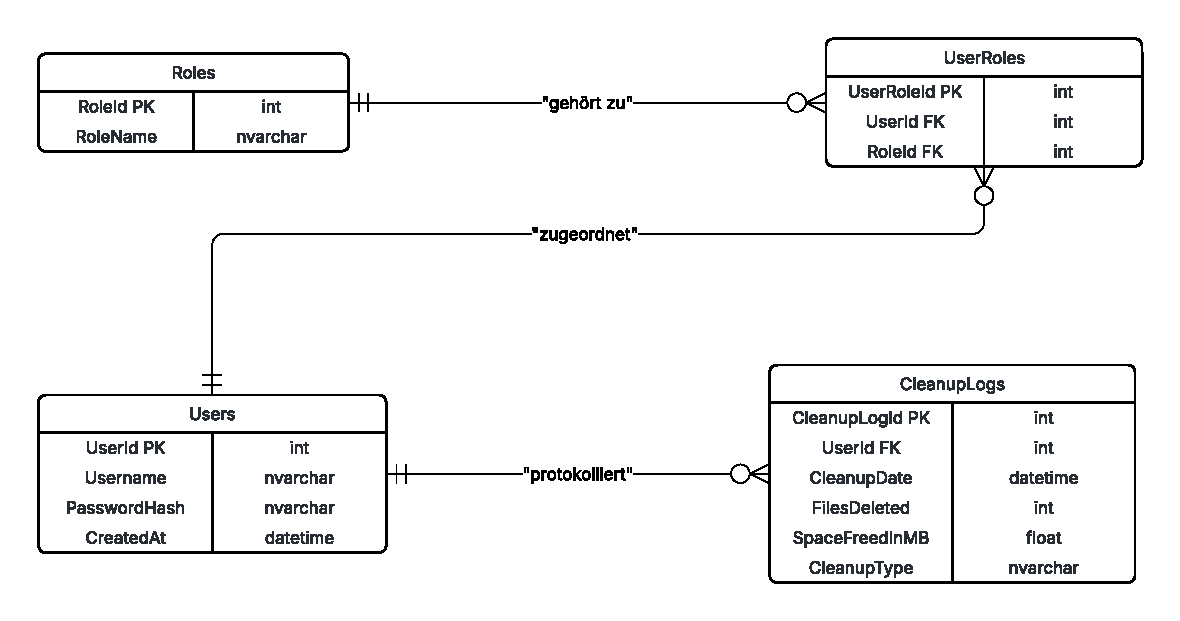
\includegraphics[width=\textwidth]{src/er_diagramm.pdf}
    \caption{ER-Diagramm der GarbageCollector-Datenbank}
\end{figure}


\setlength{\parskip}{0pt}
\setlength{\itemsep}{2pt}

\subsubsection*{Users (Benutzer)}
{\small
\begin{itemize}
    \item \textbf{UserId (PK)}: Eindeutige Kennung für jeden Benutzer.
    \item \textbf{Username}: Benutzername.
    \item \textbf{PasswordHash}: Gehashter Wert des Benutzerpassworts.
    \item \textbf{CreatedAt}: Zeitstempel bei Erstellung des Benutzers.
\end{itemize}
\textbf{Beziehungen:}
\begin{itemize}
    \item \textit{1:n} zu \textbf{CleanupLogs}: Ein Benutzer kann mehrere Bereinigungen durchgeführt haben.
    \item \textit{n:m} zu \textbf{Roles} über \textbf{UserRoles}.
\end{itemize}
}

\subsubsection*{Roles (Rollen)}
{\small
\begin{itemize}
    \item \textbf{RoleId (PK)}: Eindeutige Kennung der Rolle.
    \item \textbf{RoleName (UNQ)}: Rollenbezeichnung, z.\,B. „Admin“ oder „User“.
\end{itemize}
\textbf{Beziehung:}
\begin{itemize}
    \item \textit{1:n} zu \textbf{UserRoles}.
\end{itemize}
}

\subsubsection*{UserRoles (Benutzer-Rollen-Verknüpfung)}
{\small
\begin{itemize}
    \item \textbf{UserRoleId (PK)}: Eindeutige Kennung für jeden Eintrag.
    \item \textbf{UserId (FK)}: Verweis auf einen Benutzer.
    \item \textbf{RoleId (FK)}: Verweis auf eine Rolle.
\end{itemize}
\textbf{Beziehungen:}
\begin{itemize}
    \item \textit{n:1} zu \textbf{Users}, \textit{n:1} zu \textbf{Roles}.
\end{itemize}
}

\subsubsection*{CleanupLogs (Bereinigungsprotokolle)}
{\small
\begin{itemize}
    \item \textbf{CleanupLogId (PK)}: Eindeutige ID für den Protokolleintrag.
    \item \textbf{UserId (FK)}: Verweis auf den Benutzer.
    \item \textbf{CleanupDate}: Datum/Uhrzeit des Vorgangs.
    \item \textbf{FilesDeleted}: Anzahl gelöschter Dateien.
    \item \textbf{SpaceFreedInMB}: Freigegebener Speicherplatz in MB.
    \item \textbf{CleanupType}: Typ des Vorgangs (Standard, Junk, Duplicates).
\end{itemize}
\textbf{Beziehung:}
\begin{itemize}
    \item \textit{n:1} zu \textbf{Users}.
\end{itemize}
}

\subsection{Link zum Git-Repository}


Link zum gehosteten GitHub-Repository:

\begin{footnotesize}
\url{https://github.com/PilliPalli/Garbage-Collection-Tool-zur-Loeschung-temporaerer-Dateien}
\end{footnotesize}

Das Repository enthält:
\begin{itemize}
    \item den vollständigen Quellcode,
    \item das SQL-Skript zum Erstellen der Datenbank,
    \item eine README.md
\end{itemize}

\subsection{Testplan}


\subsection*{Testfall GC01 – Automatische Datenbereinigung}
\begin{tabular}{|p{4cm}|p{10cm}|}
\hline
 \textbf{ID:} & GC01 \\
\hline
\textbf{Beschreibung:} & Überprüfung der automatischen Datenbereinigung. \\
\hline
\textbf{Vorbedingung:} & Das Tool ist installiert, konfiguriert und der Bereinigungsprozess ist aktiviert. Es existieren alte und neue Dateien. \\
\hline
\textbf{Test-Schritte:} & 
1. Es werden Testdateien in einem temporären Verzeichnis erstellt, einige davon sind älter als der angegebene Schwellenwert (z.\,B. 10 Tage). \newline
2. Das Tool wird gestartet, und der Bereinigungsprozess ausgeführt. \newline
3. Überprüfung, ob alte Dateien entfernt wurden und neue Dateien erhalten bleiben. \\
\hline
\textbf{Erwartetes \newline Resultat:} & 
- Die alten Dateien werden erfolgreich entfernt. \newline
- Die neuen Dateien bleiben bestehen. \\
\hline
\end{tabular}

\vspace{1em}

\subsection*{Testfall GC02 – Sicherheitsfunktion (Papierkorb)}
\begin{tabular}{|p{4cm}|p{10cm}|}
\hline
\textbf{ID:} & GC02 \\
\hline
\textbf{Beschreibung:} & Test der Sicherheitsfunktion, bei der Dateien in den Papierkorb verschoben werden. \\
\hline
\textbf{Vorbedingung:} & Das Tool ist installiert und konfiguriert, und die Option zum Verschieben von Dateien in den Papierkorb ist aktiviert. \\
\hline
\textbf{Test-Schritte:} & 
1. Testdateien werden in einem temporären Verzeichnis erstellt. \newline
2. Der Bereinigungsprozess wird gestartet, und überprüft, ob die Dateien in den Papierkorb verschoben werden. \newline
3. Der Papierkorb wird auf die verschobenen Dateien überprüft. \\
\hline
\textbf{Erwartetes \newline Resultat:} & 
- Die Dateien werden nicht gelöscht, sondern in den Papierkorb verschoben. \\
\hline
\end{tabular}

\vspace{1em}

\subsection*{Testfall GC03 – Benutzerdefinierte Einstellungen}
\begin{tabular}{|p{4cm}|p{10cm}|}
\hline
\textbf{ID:} & GC03 \\
\hline
\textbf{Beschreibung:} & Test der benutzerdefinierten Einstellungen. \\
\hline
\textbf{Vorbedingung:} & Das Tool ist installiert und konfiguriert, der Bereinigungsprozess ist aktiviert. \\
\hline
\textbf{Test-Schritte:} & 
1. Zugriff auf die Einstellungsoptionen des Tools. \newline
2. Anpassung der Parameter in der Konfigurationsdatei (z.B. Verzeichnis, Dateimuster, Alter der zu löschenden Dateien). \newline
3. Ausführung des Bereinigungsprozesses und Überprüfung, ob die Änderungen korrekt umgesetzt wurden. \\
\hline
\textbf{Erwartetes \newline Resultat:} & 
- Die neuen Einstellungen werden korrekt angewendet. \newline
- Der Bereinigungsprozess arbeitet entsprechend den benutzerdefinierten Einstellungen. \\
\hline
\end{tabular}

\vspace{1em}

\subsection*{Testfall GC04 – Duplikatentfernung}
\begin{tabular}{|p{4cm}|p{10cm}|}
\hline
\textbf{ID:} & GC04 \\
\hline
\textbf{Beschreibung:} & Test der Duplikatentfernung. \\
\hline
\textbf{Vorbedingung:} & Doppelte Dateien befinden sich im Verzeichnis. \\
\hline
\textbf{Test-Schritte:} & 
1. Erstellen von doppelten Dateien (gleicher Inhalt, unterschiedlicher Dateiname). \newline
2. Start des Bereinigungsprozesses. \newline
3. Überprüfung, ob die Duplikate entfernt werden und nur eine Datei bestehen bleibt. \\
\hline
\textbf{Erwartetes \newline Resultat:} & 
- Nur eine Kopie jeder doppelten Datei bleibt bestehen. \\
\hline
\end{tabular}

\vspace{1em}

\subsection*{Testfall GC05 – Passwortänderung}
\begin{tabular}{|p{4cm}|p{10cm}|}
\hline
\textbf{ID:} & GC05 \\
\hline
\textbf{Beschreibung:} & Überprüfung der Passwortänderungsfunktion. \\
\hline
\textbf{Vorbedingung:} & Der Benutzer ist eingeloggt, und es gibt einen Testbenutzer mit einem bekannten Passwort. \\
\hline
\textbf{Test-Schritte:} & 
1. Zugriff auf die Einstellungen, um das Passwort zu ändern. \newline
2. Eingeben des aktuellen Passworts, gefolgt von einem neuen Passwort. \newline
3. Überprüfen, ob die Passwortänderung korrekt durchgeführt wurde. \\
\hline
\textbf{Erwartetes \newline Resultat:} & 
- Das Passwort wird erfolgreich geändert. \\
\hline
\end{tabular}


\newpage
\subsection{Unit Tests}
Aktuell ist die Implementierung von Unit-Tests nicht geplant. Stattdessen wird der Fokus auf manuelle Tests gelegt, um sicherzustellen, dass die Schlüsselkomponenten des Tools wie erwartet funktionieren. Manuelle Tests werden für kritische Funktionen durchgeführt.

Eine spätere Einführung von Unit-Tests bleibt optional, abhängig von den zukünftigen Anforderungen und der Projektentwicklung.

\vspace{1em}
\textbf{Begründung:}
\begin{enumerate}
    \item \textbf{Kein Verzicht auf Qualitätssicherung:} \\
    Statt automatisierter Tests werden manuelle Tests für zentrale Funktionen priorisiert.
    
    \item \textbf{Flexibilität für die Zukunft:} \\
    Die Möglichkeit zur Einführung von Unit-Tests bleibt offen, falls sich Anforderungen oder Ressourcen ändern.
    
    \item \textbf{Zeitmanagement:} \\
    Fokus auf funktionierende Hauptfunktionen, anstatt zusätzliche Komplexität durch Tests hinzuzufügen.
\end{enumerate}


% 2. Benutzerhandbuch
\section{Benutzerhandbuch}
\subsection{Start und Anmeldung}


Nach dem Start der Anwendung wird der Benutzer direkt zum Anmeldebildschirm weitergeleitet. Dort kann sich ein bestehender Nutzer mit seinem Benutzernamen und Passwort anmelden. Alternativ kann über den Link \glqq Registrierung\grqq{} ein neuer Account erstellt werden.

\begin{figure}[H]
    \centering
    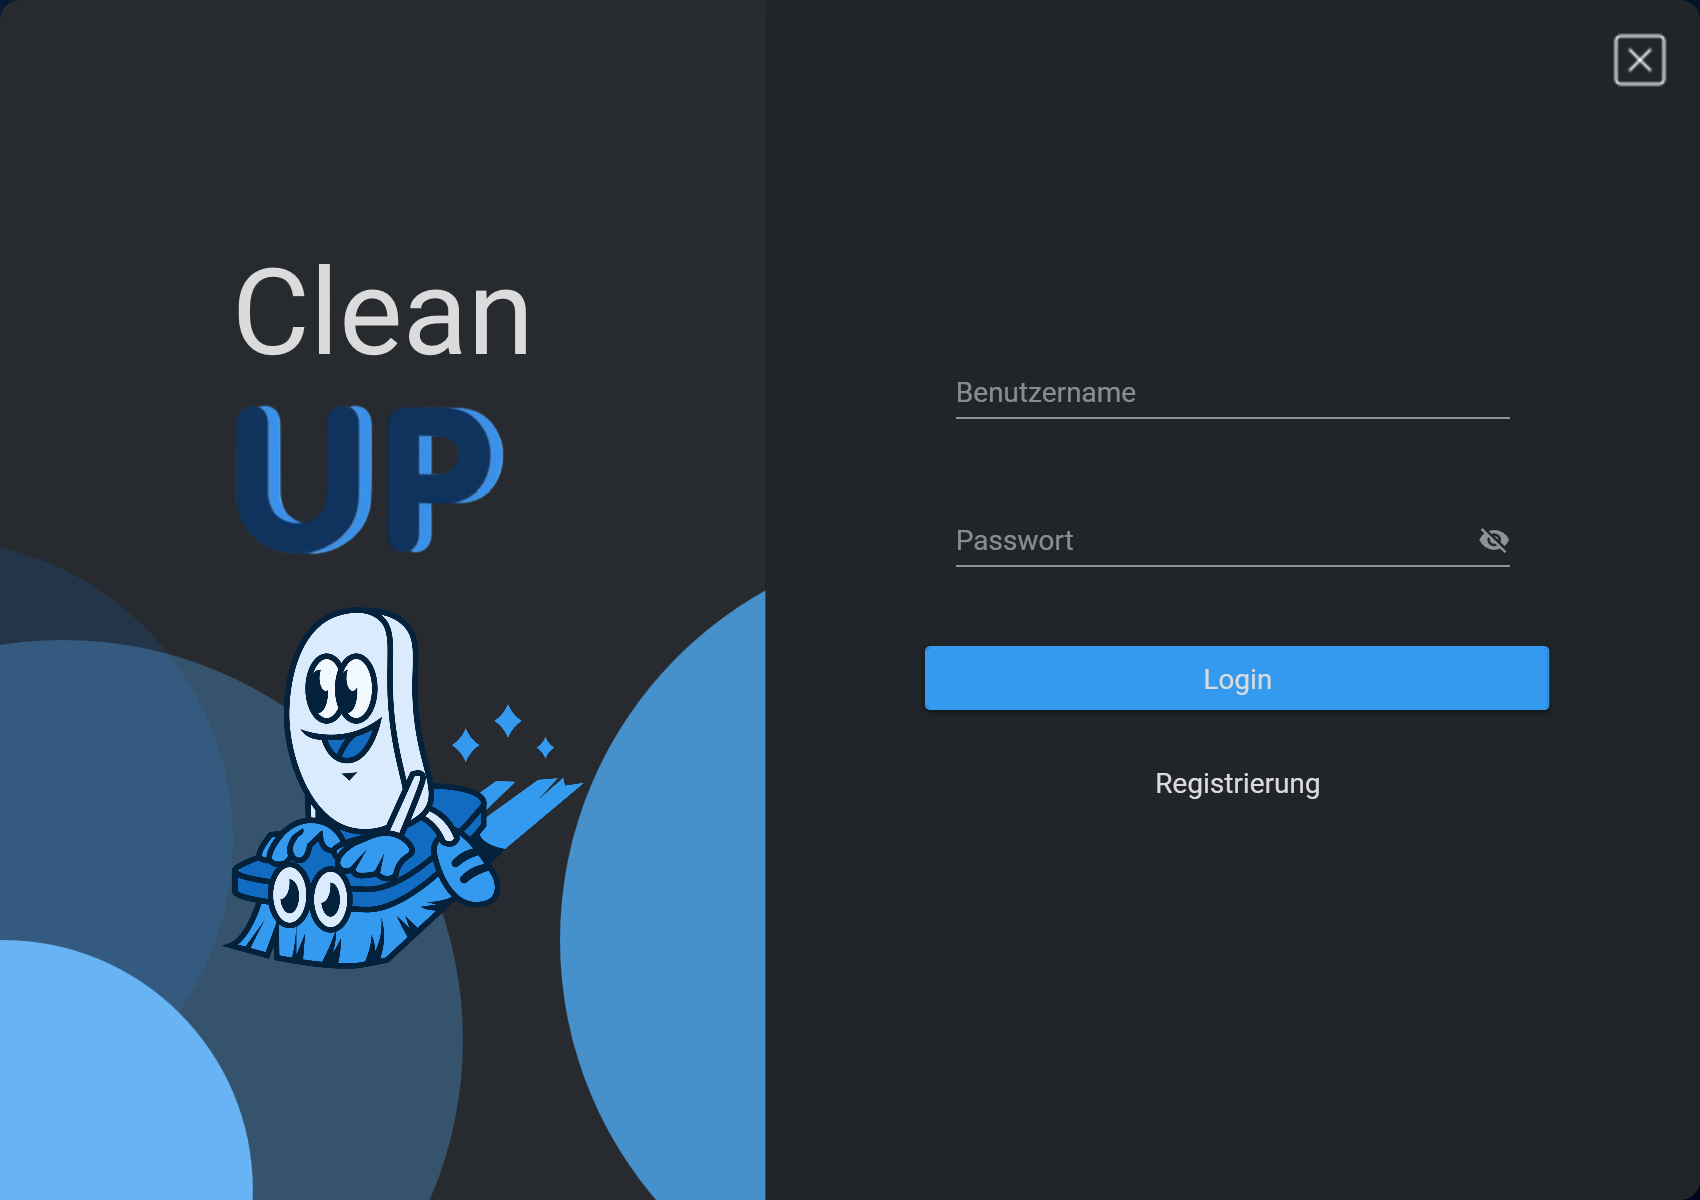
\includegraphics[width=0.8\textwidth]{src/screenshot_login.png}
    \caption{Login-Maske mit Eingabefeldern für Benutzername und Passwort}
\end{figure}

Bei der Registrierung müssen ein Benutzername sowie ein sicheres Passwort (mindestens 8 Zeichen) eingegeben und bestätigt werden. Das System überprüft die Eingaben und gibt bei fehlerhafter Eingabe eine visuelle Rückmeldung. Nach erfolgreicher Registrierung wird eine grüne Bestätigung angezeigt. Der Benutzer kann anschließend über den Link \glqq Zurück zum Login\grqq{} zum Anmeldebildschirm zurückkehren und sich mit den zuvor gewählten Anmeldedaten einloggen.

\begin{figure}[H]
    \centering
    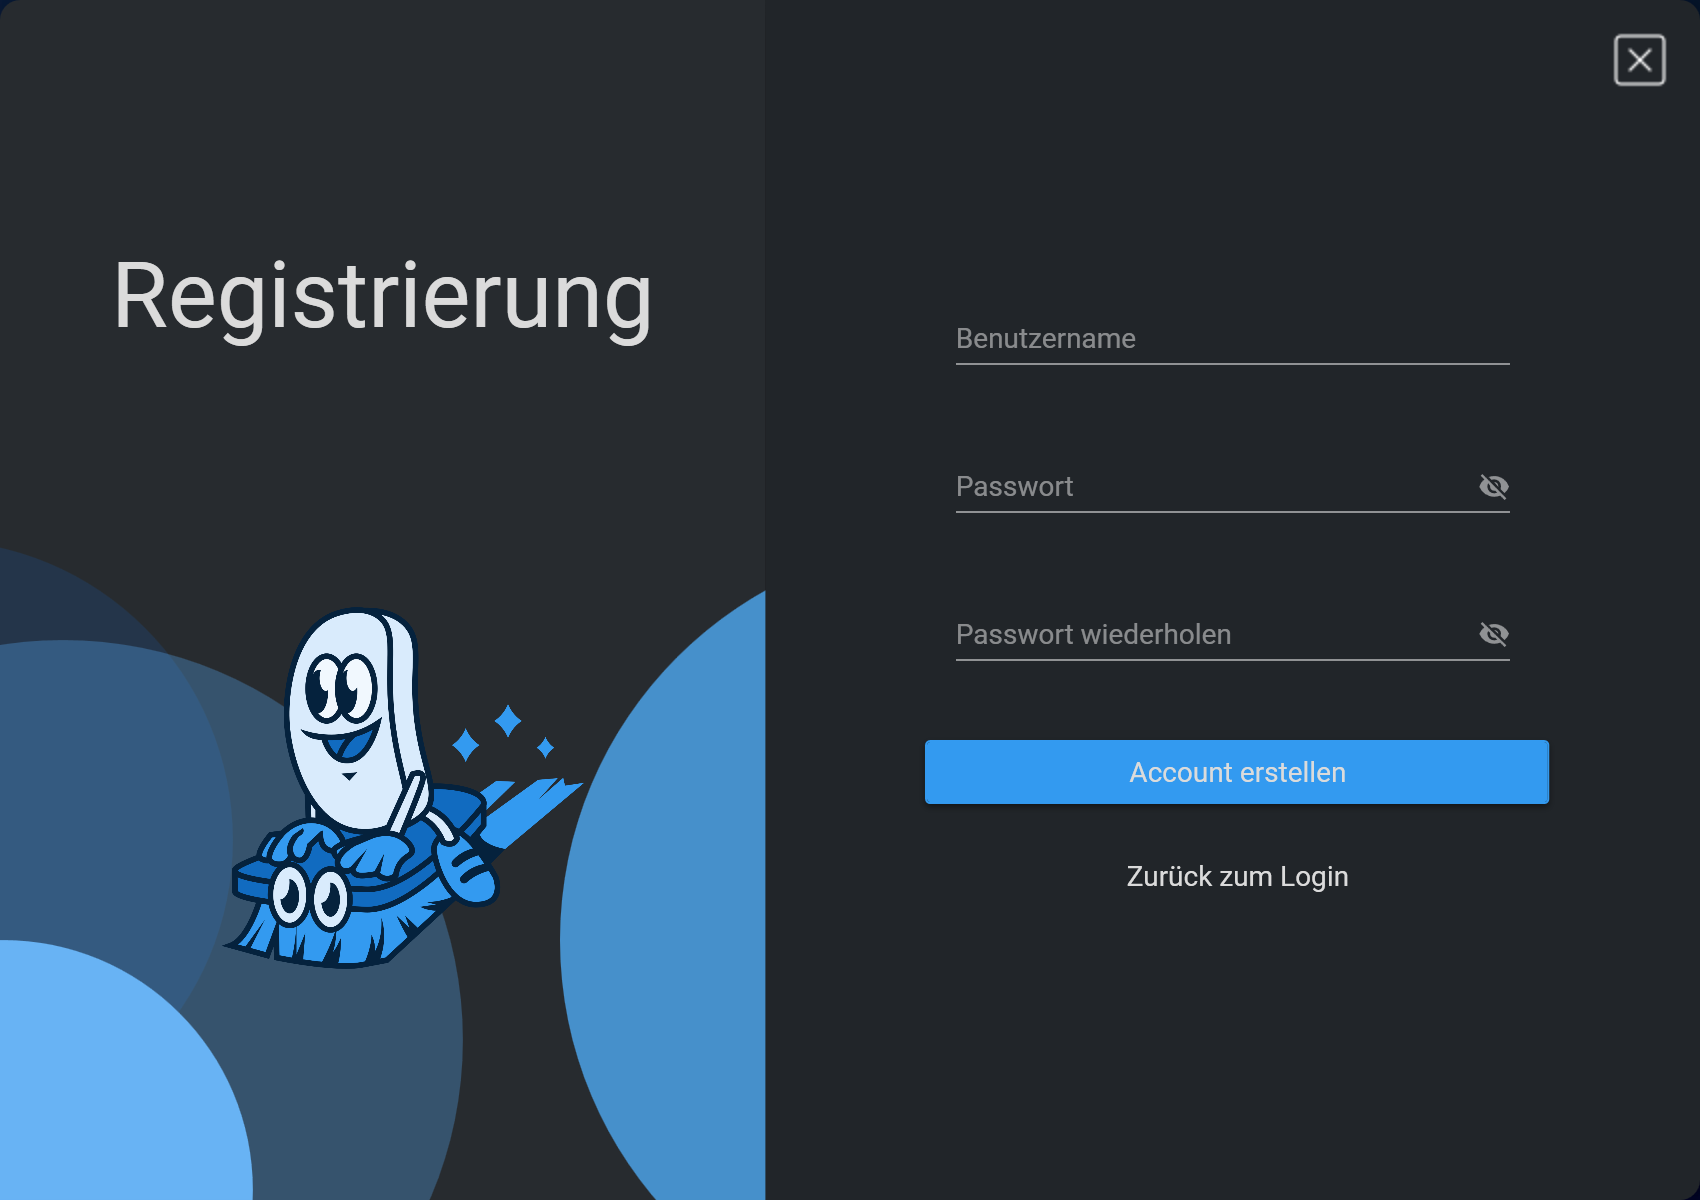
\includegraphics[width=0.8\textwidth]{src/screenshot_register.png}
    \caption{Registrierungsformular mit Passwortbestätigung}
\end{figure}

Nach erfolgreicher Anmeldung wird der Benutzer auf den Home-Bildschirm der Anwendung weitergeleitet und dort mit einer persönlichen Willkommensnachricht begrüßt. Zusätzlich werden ihm Statistiken zur Anwendung angezeigt, darunter die Gesamtanzahl gelöschter Dateien, der freigegebene Speicherplatz sowie eine Historie der letzten fünf durchgeführten Bereinigungsvorgänge. 

Bei Bedarf kann der Nutzer seine gesamte Historie einsehen, indem er seine Statistiken über den Button \glqq Logs exportieren\grqq{} als \texttt{.csv}-Datei herunterlädt. Auf Wunsch können die Statistiken auch vollständig zurückgesetzt und gelöscht werden. 

Über das Menü, welches als Sidebar umgesetzt wurde, kann der Nutzer nach Belieben zwischen den einzelnen Ansichten hin- und herwechseln.

\begin{figure}[H]
    \centering
    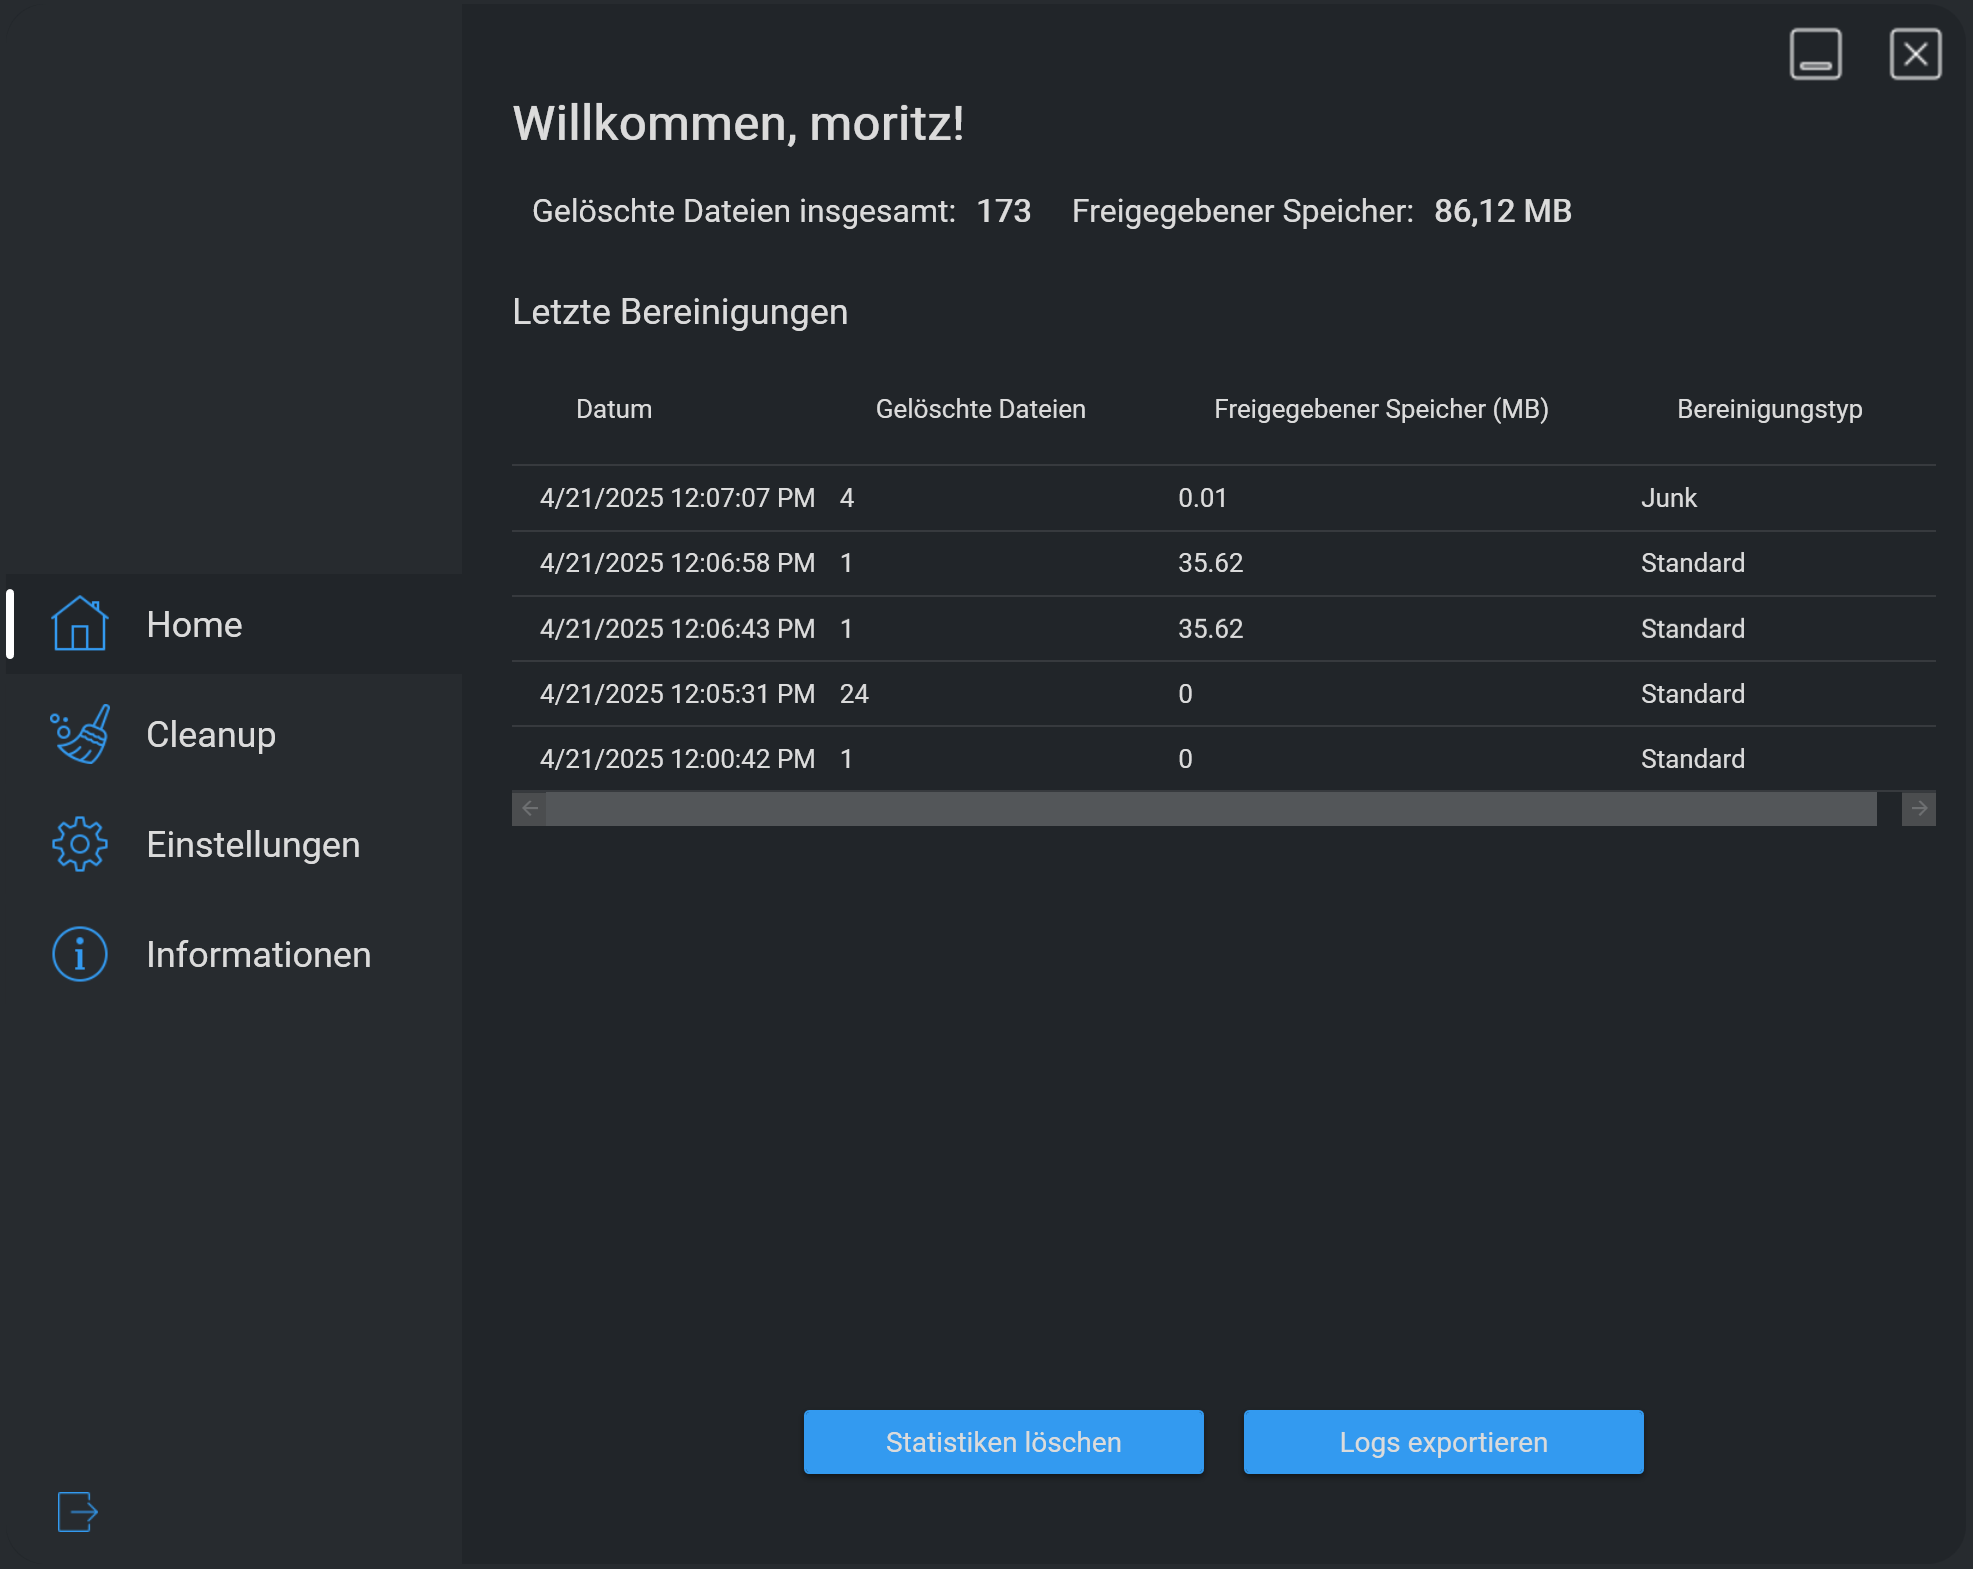
\includegraphics[width=0.9\textwidth]{src/screenshot_home.png}
    \caption{Home-Bildschirm des Nutzers mit dem gesetzten Benutzernamen \glqq moritz\grqq{}}
\end{figure}



\subsection{Einstellungen konfigurieren}

Über die Navigationsleiste auf der linken Seite kann der Benutzer die Einstellungen aufrufen. In diesem Bereich lassen sich verschiedene Verhaltensweisen der Anwendung anpassen.

\begin{itemize}
    \item \textbf{Dateien direkt löschen:} Wenn diese Option aktiviert ist, werden erkannte Dateien unmittelbar entfernt. Ist sie deaktiviert, landen die Dateien zunächst im Papierkorb, was eine Wiederherstellung ermöglicht.
    \item \textbf{Rekursiv löschen:} Diese Option bestimmt, ob auch Unterordner des angegebenen Verzeichnisses durchsucht und bereinigt werden sollen.
\end{itemize}

Zusätzlich besteht die Möglichkeit, das Benutzerpasswort zu ändern. Dazu muss zunächst das aktuelle Passwort eingegeben werden, gefolgt von der Eingabe und Bestätigung eines neuen Passworts. Das System prüft, ob das neue Passwort den Sicherheitsrichtlinien entspricht und ob beide Eingaben übereinstimmen.

\begin{figure}[H]
    \centering
    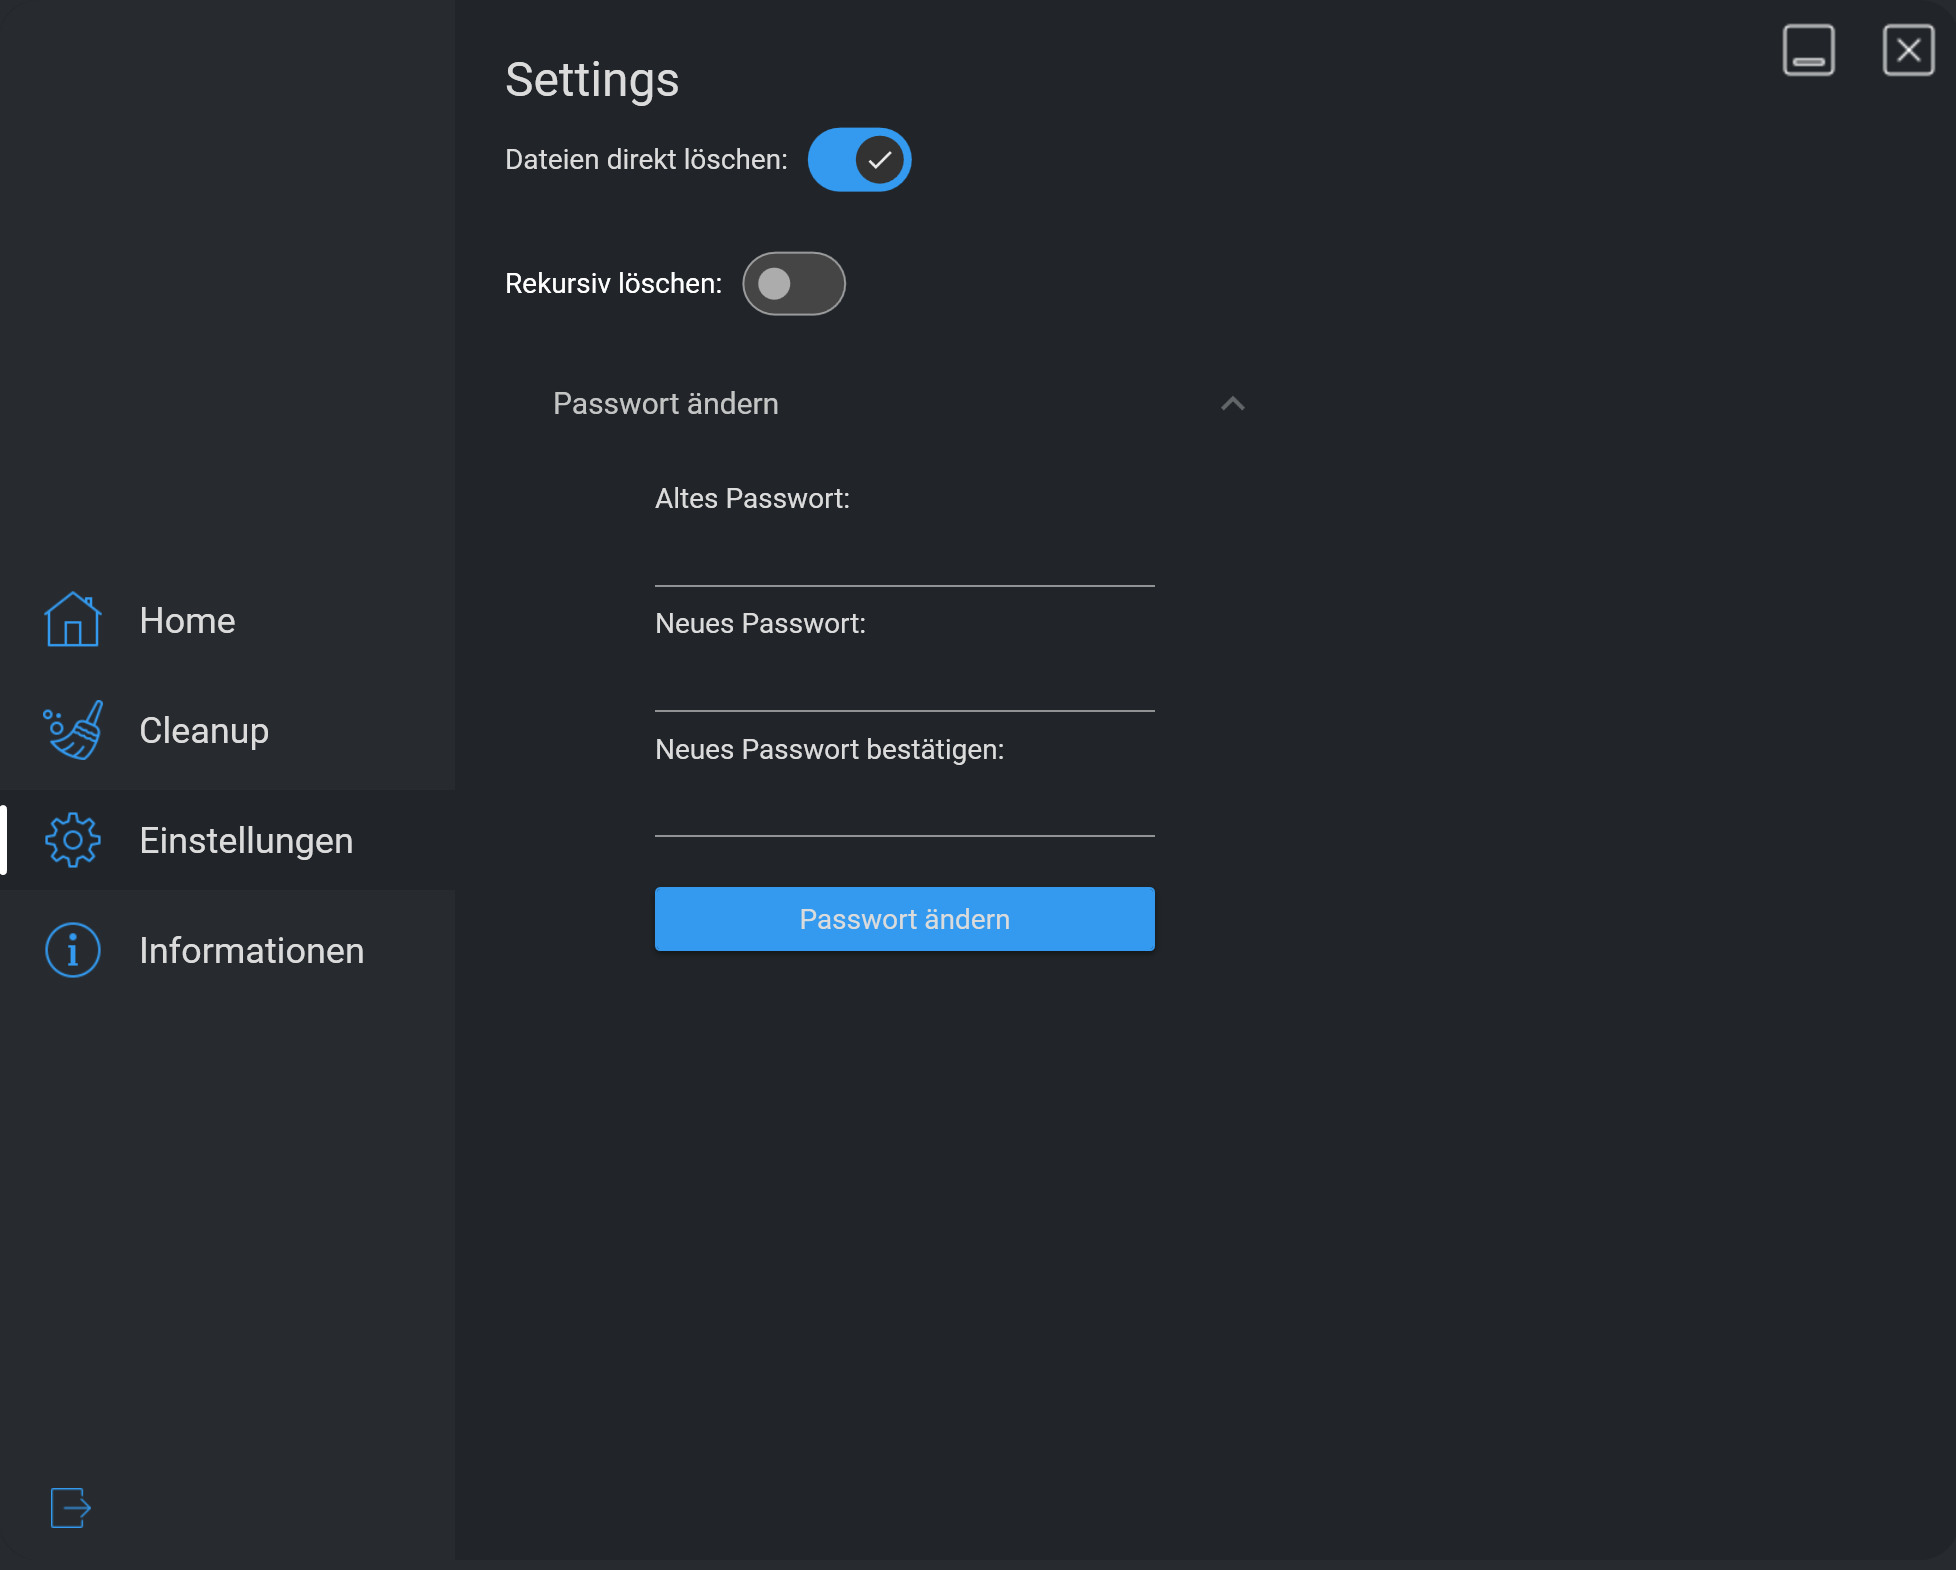
\includegraphics[width=0.9\textwidth]{src/screenshot_settings.png}
    \caption{Einstellungsseite mit Optionen zur Konfiguration und Passwortänderung}
\end{figure}



\subsection{Bereinigungsfunktionen}


Über den Menüpunkt \glqq Cleanup\grqq{} gelangt der Nutzer zur zentralen Funktionalität der Anwendung: dem Löschen temporärer und überflüssiger Dateien. In diesem Bereich kann der Benutzer gezielt konfigurieren, welche Dateien gelöscht werden sollen und in welchem Ordner die Bereinigung erfolgen soll.

\begin{itemize}
    \item \textbf{Pfad des Ordners:} Angabe des zu bereinigenden Verzeichnisses.
    \item \textbf{Älter als (Tage):} Legt fest, wie alt Dateien mindestens sein müssen, um als löschwürdig zu gelten.
    \item \textbf{Dateimuster:} Ermöglicht die Einschränkung der Löschung auf bestimmte Dateitypen (z.\,B. \texttt{*.tmp, *.log}); auch einzelne Dateien können gezielt gefiltert werden.
\end{itemize}

Der Pfad des Ordners muss nicht manuell eingegeben werden, sondern kann auch über den Button links neben dem Eingabefeld ausgewählt werden. Hierbei öffnet sich ein Dialogfenster (Windows-Explorer), über das der gewünschte Zielpfad bequem ausgewählt werden kann.

\vspace{1em}
Dem Benutzer stehen drei Buttons zur Verfügung:

\begin{itemize}
    \item \textbf{Clean Up:} Startet die Standard-Bereinigung gemäß der angegebenen Kriterien.
    \item \textbf{Junk Files löschen:} Sucht gezielt nach typischen temporären oder nutzlosen Dateien und entfernt diese.
    \item \textbf{Duplikate löschen:} Erkennt und entfernt doppelt vorhandene Dateien im gewählten Verzeichnis. Wichtig ist, dass nur die Duplikate gelöscht werden – die zuerst gefundene Originaldatei bleibt erhalten.
\end{itemize}

\vspace{1em}
Darunter befindet sich der Bereich \textbf{Scheduler-Einstellungen}. Hier kann der Benutzer ein automatisches Cleanup-Intervall (in Minuten) festlegen. Die Anwendung führt dann selbstständig in regelmäßigen Abständen eine Bereinigung durch.

\begin{itemize}
    \item \textbf{Scheduler starten:} Aktiviert die automatische Bereinigung.
    \item \textbf{Scheduler stoppen:} Deaktiviert den geplanten Bereinigungsprozess.
\end{itemize}

Eine Statusanzeige informiert den Nutzer darüber, wann die nächste automatische Bereinigung stattfinden wird oder ob der Vorgang bereits abgeschlossen ist.

\begin{figure}[H]
    \centering
    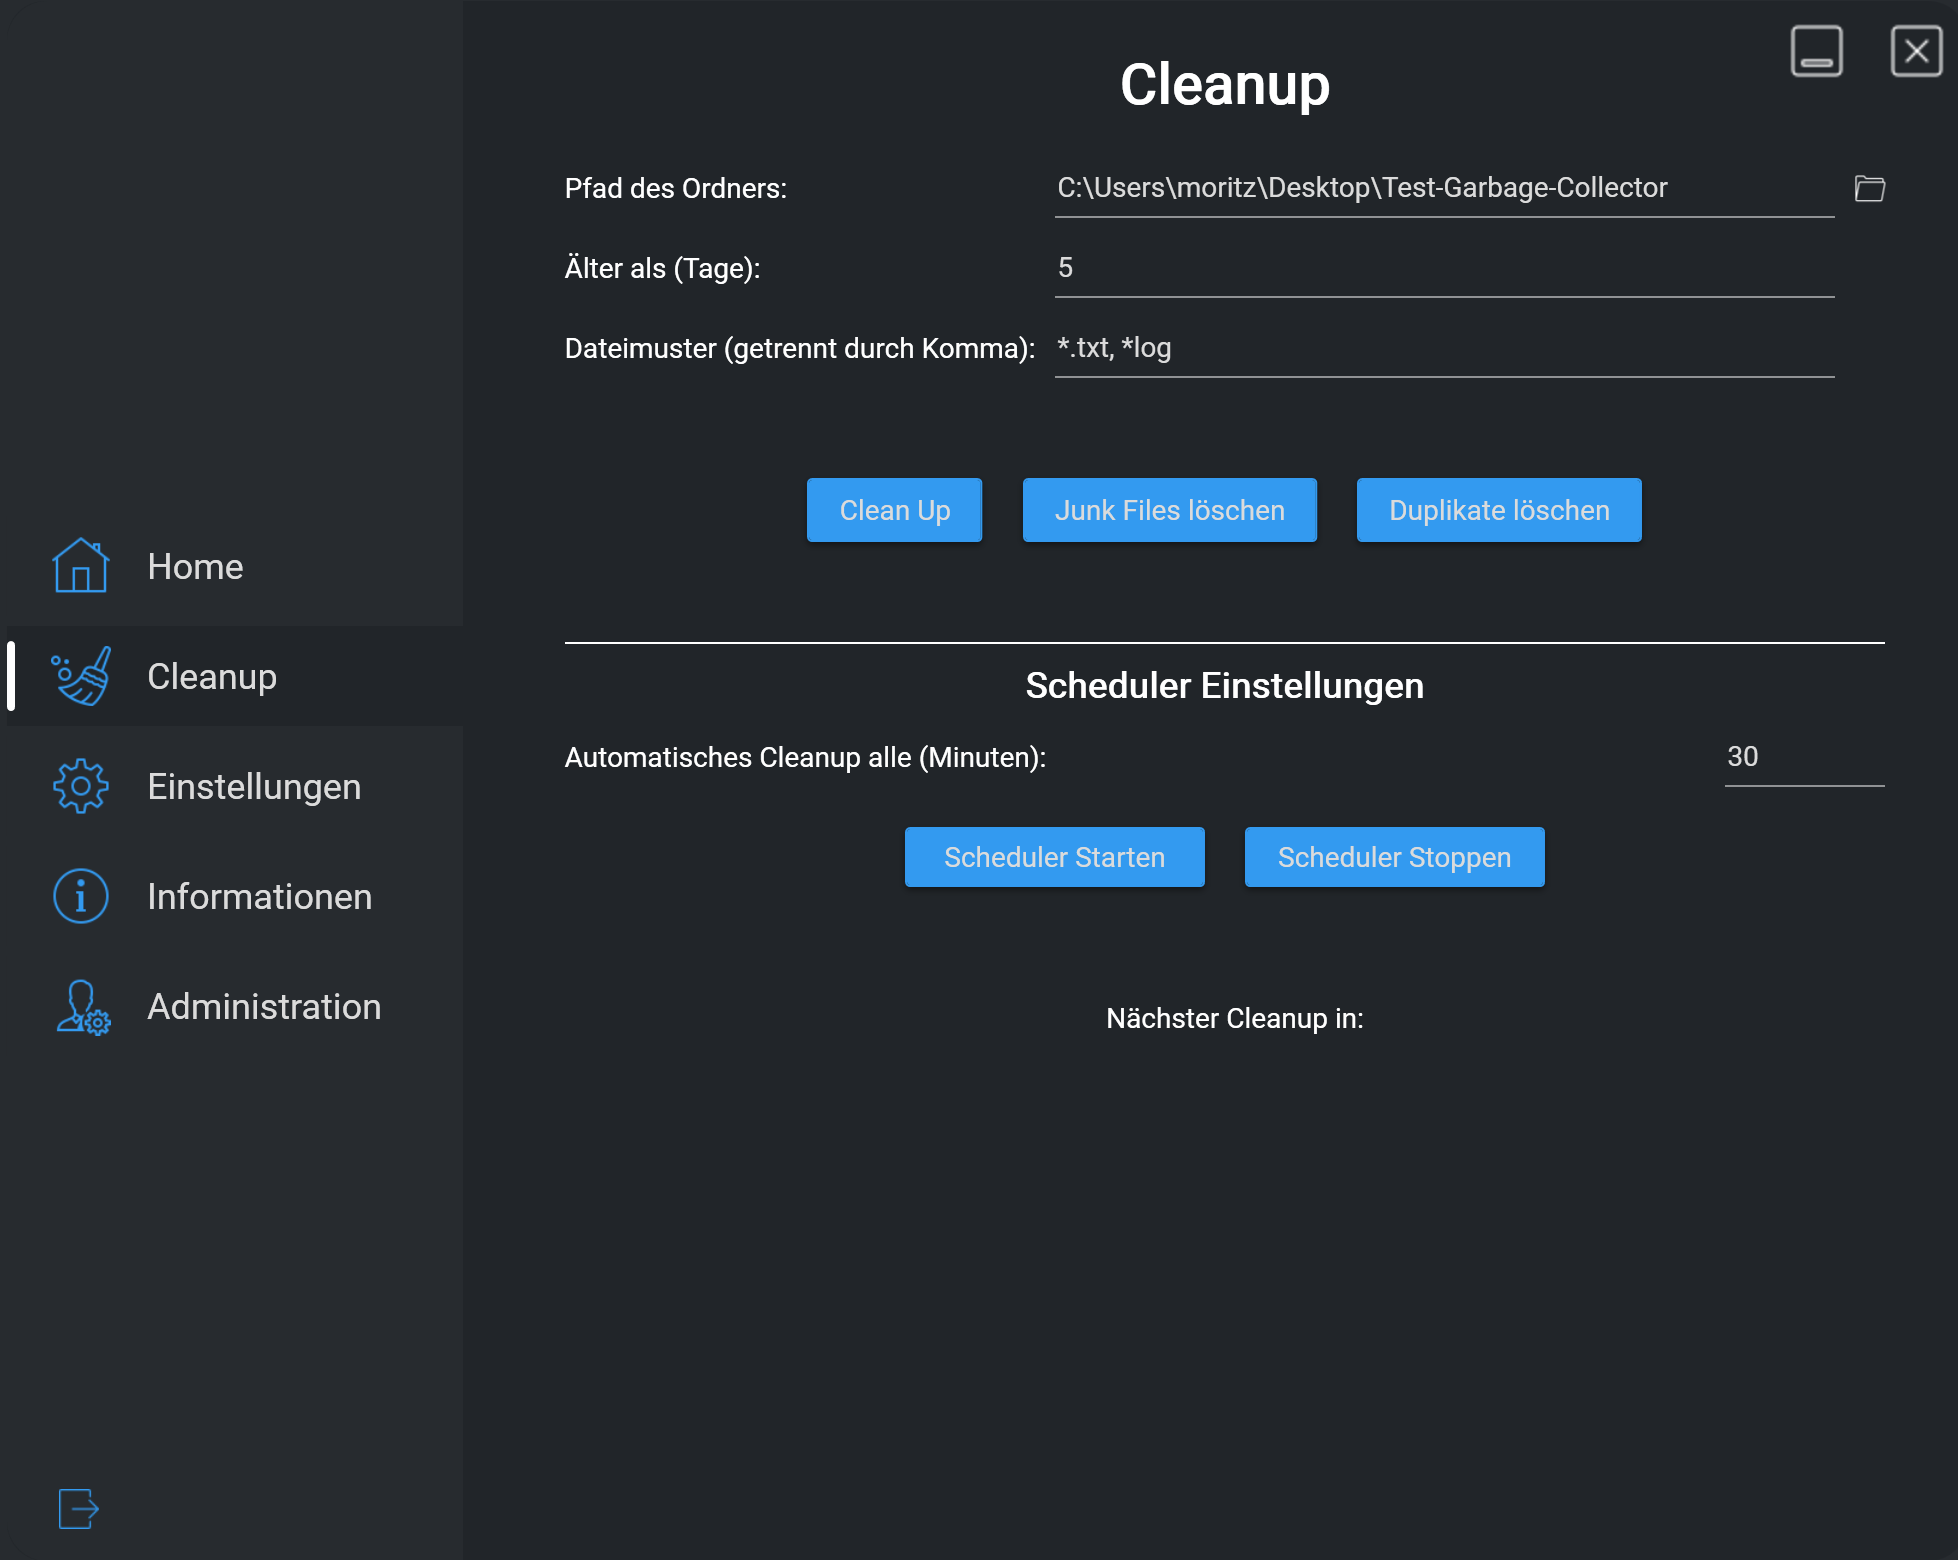
\includegraphics[width=0.9\textwidth]{src/screenshot_cleanup.png}
    \caption{Cleanup-Seite mit Optionen zur manuellen und automatischen Bereinigung}
\end{figure}

Im folgenden Screenshot ist die Bereinigungsfunktion inklusive laufendem Scheduler in Aktion zu sehen. Der Benutzer wird in Echtzeit über den Bereinigungsprozess informiert – inklusive Fortschrittsbalken und Anzeige der aktuell gelöschten Datei samt Pfadangabe. Während der Bereinigung sind alle Buttons deaktiviert (ausgegraut), um gleichzeitige Aktionen zu verhindern. Der Scheduler zeigt präzise an, wann der nächste automatische Cleanup durchgeführt wird.

\begin{figure}[H]
    \centering
    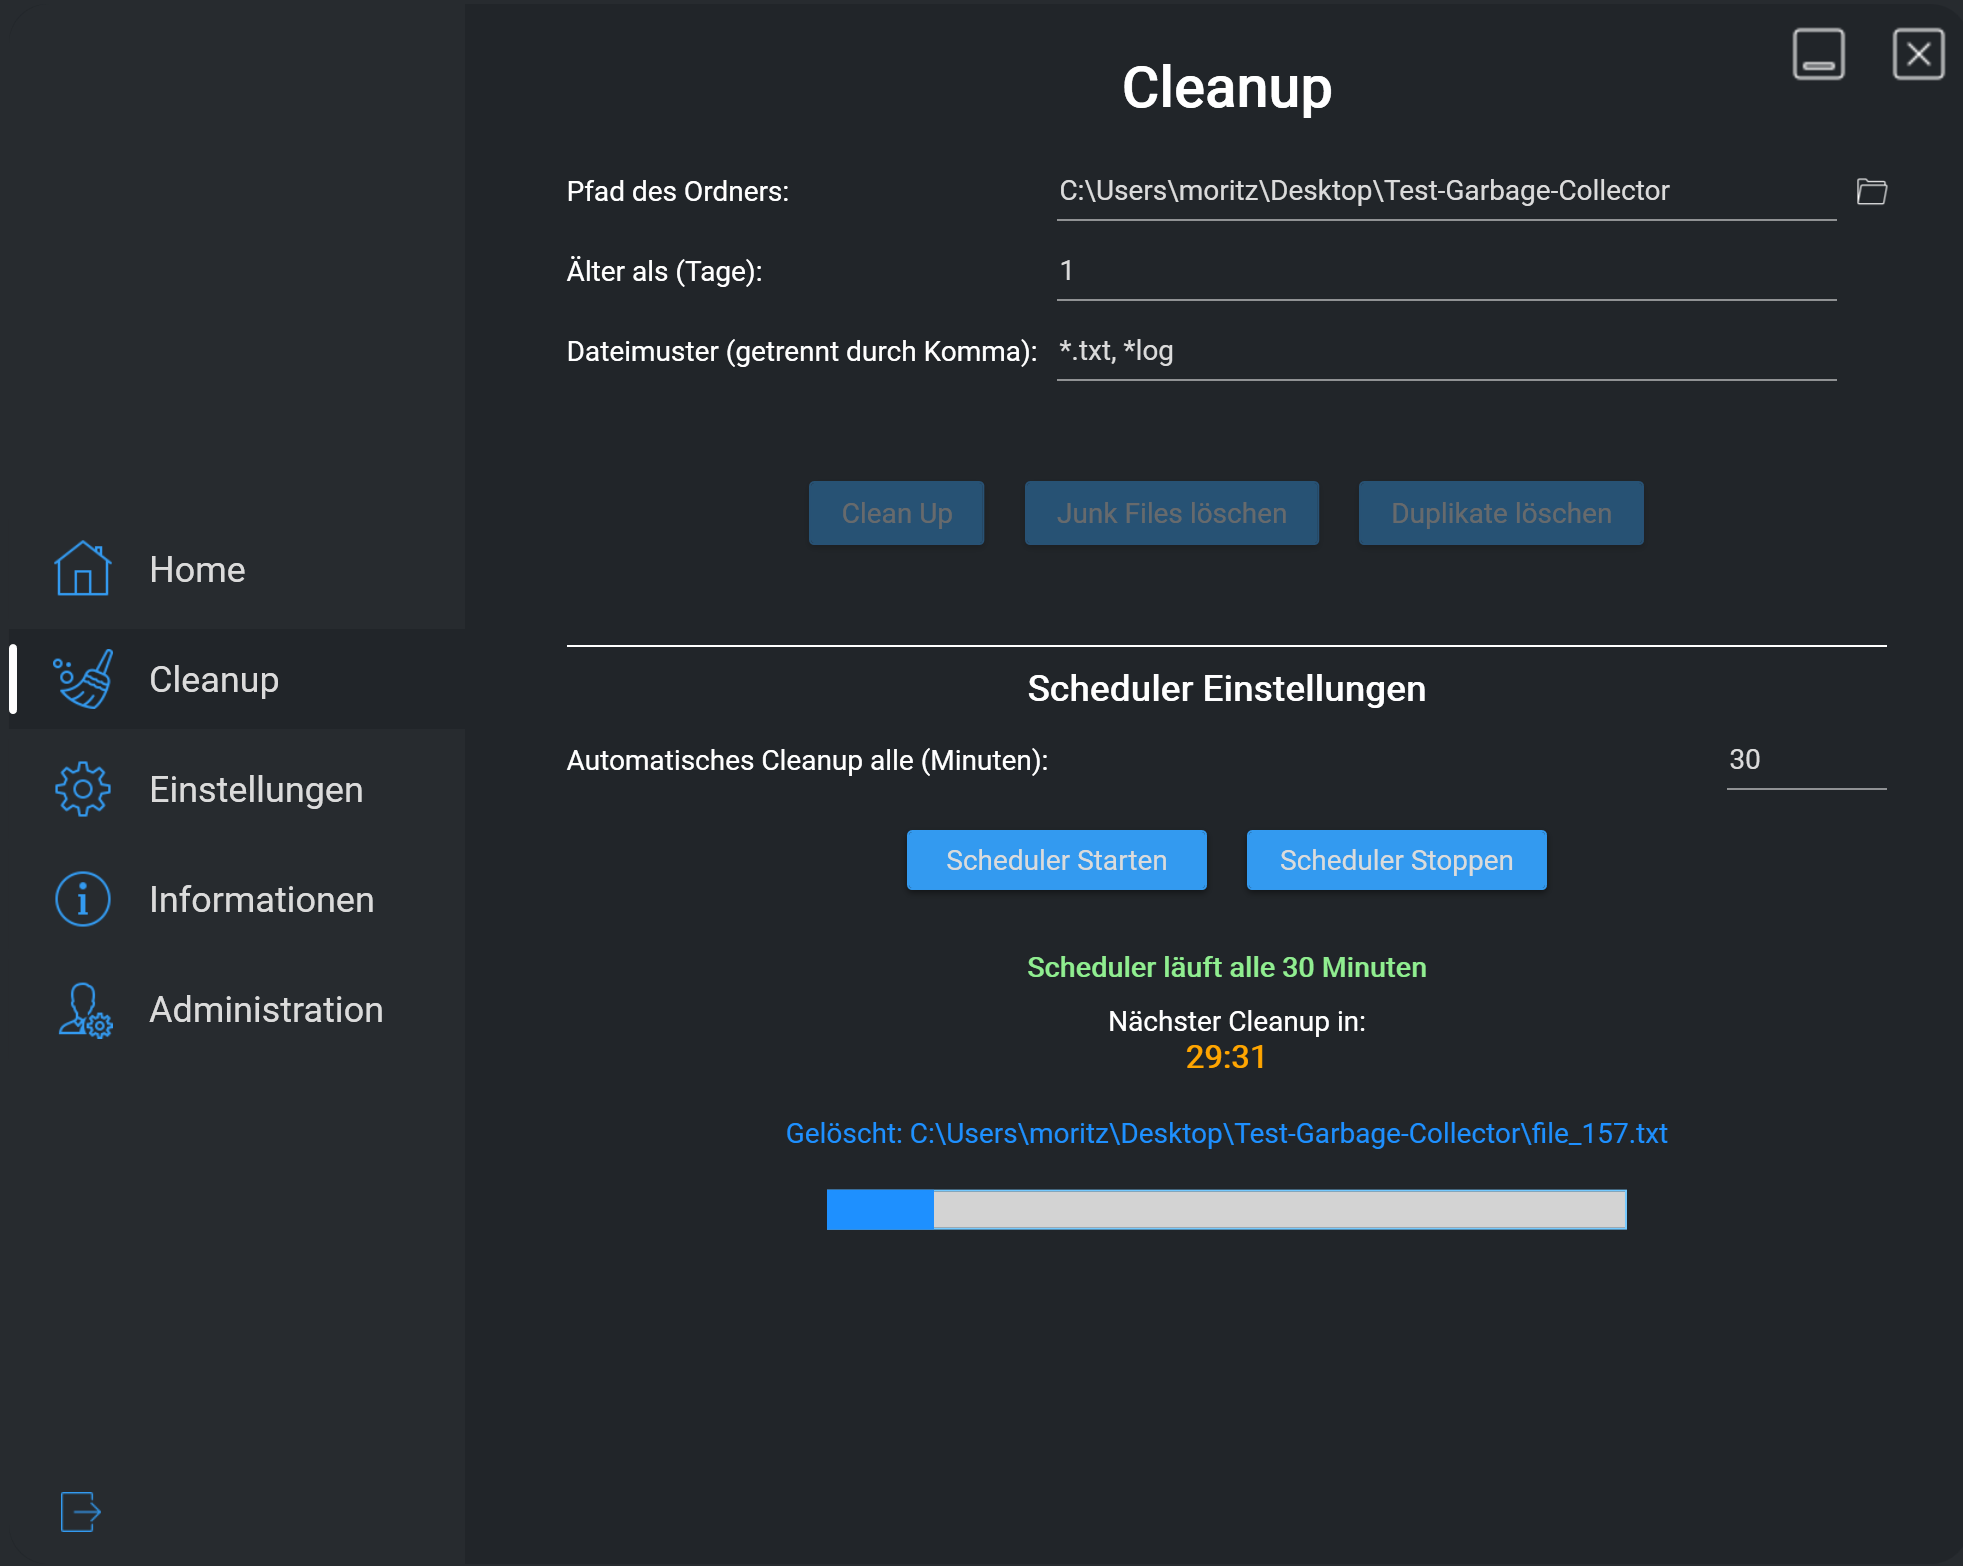
\includegraphics[width=0.9\textwidth]{src/screenshot_action.png}
    \caption{Cleanup-Seite mit laufendem Bereinigungsprozess und aktivem Scheduler}
\end{figure}

\vspace{1em}
Da es sich um ein konfigurationsdateigesteuertes Programm handelt, können die meisten Einstellungen auch direkt über eine Konfigurationsdatei (\texttt{config.json}) vorgenommen werden. Diese Datei wird beim ersten Start automatisch im Programmverzeichnis mit Beispieldaten angelegt und bleibt stets synchron mit den Einstellungen der Benutzeroberfläche.Auch der Connection String zur Datenbank lässt sich dort zentral anpassen. Details zur internen Handhabung und zur Konfiguration der Datenbankverbindung sind im Kapitel  \hyperref[sec:03_02_datenbankanbindung_und_docker]{\textbf{3.2 Datenbankanbindung und Docker}} erläutert.

\begin{figure}[H]
    \centering
    \begin{jsoncode}
{
  "SearchPath": "C:\\Users\\moritz\\Desktop\\Test-Garbage-Collector",
  "FilePatterns": [
    "*.txt"
  ],
  "OlderThanDays": 5,
  "DeleteDirectly": true,
  "DeleteRecursively": false,
  "ConnectionString": "Data Source=192.168.178.111;Initial Catalog=GarbageCollectorDB;"
}
\end{jsoncode}
    \caption{Beispiel einer möglichen \texttt{config.json}}
\end{figure}
% \begin{figure}[H]
%     \centering
%     \includegraphics[width=0.9\textwidth]{src/configjson_code.png}
%     \caption{Beispiel einer möglichen \texttt{config.json}}
% \end{figure}




\subsection{Administration}


Benutzer mit Administratorrechten haben Zugriff auf den Menüpunkt \glqq Administration\grqq{}, über den sie die Benutzerverwaltung der Anwendung steuern können. 

In der Übersicht werden alle registrierten Benutzer angezeigt, inklusive:

\begin{itemize}
    \item \textbf{Benutzername}
    \item \textbf{Erstellt am (Zeitstempel)}
    \item \textbf{Rolle} (z.\,B. \texttt{Admin} oder \texttt{User})
\end{itemize}

\vspace{0.5em}
Folgende Funktionen stehen zur Verfügung:

\begin{itemize}
    \item \textbf{Benutzer löschen:} Entfernt den ausgewählten Benutzer dauerhaft aus dem System.
    \item \textbf{Passwort zurücksetzen:} Setzt das Passwort des ausgewählten Benutzers auf \glqq defaultPassword\grqq{} zurück. Nach dem Login kann der Benutzer das Passwort über die Einstellungen ändern.
    \item \textbf{Rolle zuweisen:} Ermöglicht die Zuweisung einer neuen Rolle (z.\,B. \texttt{Admin} oder \texttt{User}) an den ausgewählten Benutzer.
\end{itemize}

Diese Funktionen sind ausschließlich für Administratoren verfügbar und ermöglichen eine zentrale und sichere Verwaltung der Benutzerkonten.

Besondere Regeln gelten für zwei spezielle Fälle:

\begin{itemize}
    \item Der \textbf{erste registrierte Benutzer} erhält automatisch die Rolle \texttt{Admin}.
    \item Der Benutzer mit dem festen Benutzernamen \texttt{admin} ist dauerhaft Administrator und kann aus Sicherheitsgründen weder bearbeitet noch gelöscht werden.
\end{itemize}

Diese Schutzmechanismen stellen sicher, dass stets mindestens ein voll berechtigter Administrator vorhanden ist, der die vollständige Kontrolle über das System behält.

\begin{figure}[H]
    \centering
    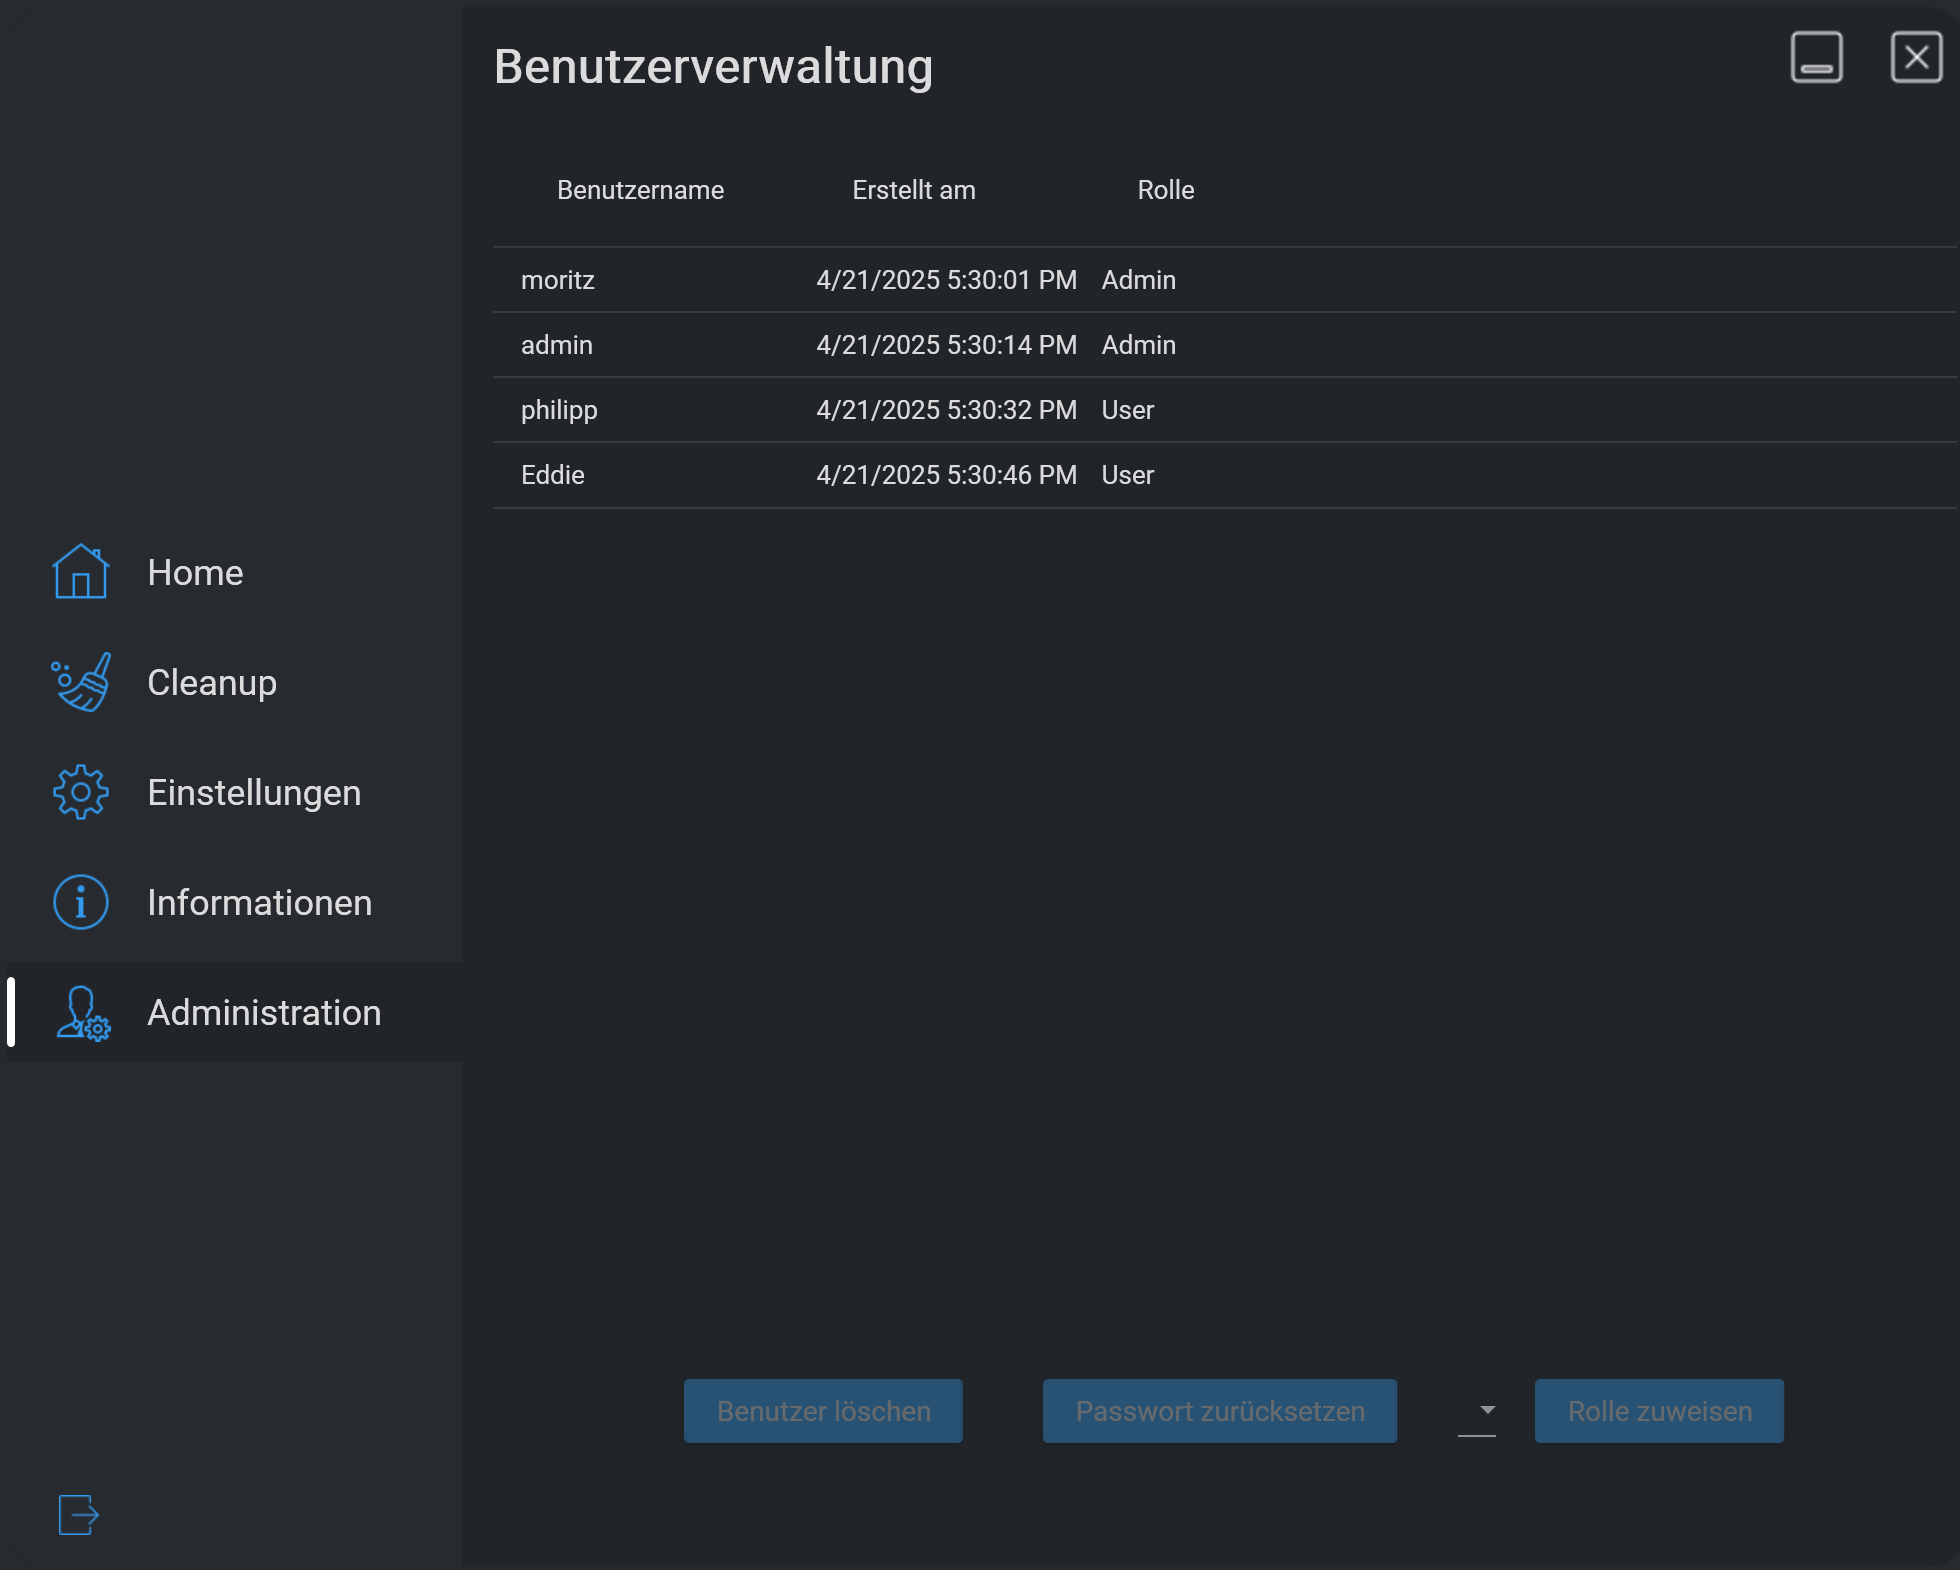
\includegraphics[width=0.9\textwidth]{src/screenshot_admin.png}
    \caption{Administrationsbereich zur Benutzerverwaltung mit Rollenzuweisung}
\end{figure}


\subsection{Abmeldung und Beenden}


Im rechten oberen Bereich der Anwendung befinden sich zwei Buttons zur Fenstersteuerung:

\begin{itemize}
    \item \textbf{Minimieren:} Reduziert das Fenster in die Taskleiste.
    \item \textbf{Schließen:} Beendet die Anwendung vollständig.
\end{itemize}

Am unteren linken Rand der Navigation befindet sich der Button zum Ausloggen. Dieser ermöglicht es dem Benutzer, die aktuelle Sitzung zu beenden und sich anschließend mit einem anderen Benutzerkonto neu anzumelden.

\subsection*{Hinweis zur Informationsseite}

Über die Menüoption \glqq Informationen\grqq{} kann eine kompakte Bedienhilfe innerhalb der Anwendung aufgerufen werden. Diese enthält in Kurzform die wichtigsten Funktionen und Anwendungsbereiche der Software. Die Informationsseite dient als unterstützende Hilfe für neue Nutzer oder zur schnellen Auffrischung der Funktionsweise.



% 3. Implementierung
\section{Implementierung}
\subsection{Architekturüberblick}
\input{kapitel/03_01_architekturüberblick}

\subsection{Datenbankanbindung und Docker}
Für die Speicherung von Benutzerdaten, Rollen, Protokollen sowie Konfigurationen wird eine relationale Datenbank auf Basis von \textbf{Microsoft SQL Server} eingesetzt. Die Anbindung erfolgt über \textbf{Entity Framework Core}, wodurch eine objektorientierte Kommunikation mit der Datenbank möglich ist. Die Datenbankmodelle – beispielsweise \texttt{User}, \texttt{CleanupLog} oder \texttt{Role} – sind als C\#-Klassen im Projekt umgesetzt und werden über einen zentralen \texttt{DbContext} verwaltet.

\subsubsection*{Entwicklungsumgebung mit Docker}

Während der Entwicklung kommt \textbf{Docker} zum Einsatz, um die Datenbank in einem isolierten Container bereitzustellen. Dies bietet mehrere Vorteile:

\begin{itemize}
    \item \textbf{Plattformunabhängigkeit:} Die Umgebung lässt sich auf jedem System mit Docker identisch starten.
    \item \textbf{Reproduzierbarkeit:} Fehler durch unterschiedliche Systemkonfigurationen werden minimiert.
    \item \textbf{Schnelles Setup:} Die gesamte Datenbank ist mit einem einzigen Befehl einsatzbereit.
    \item \textbf{Isolierte Testumgebung:} Änderungen an der Datenbankstruktur können risikolos getestet werden.
\end{itemize}

\begin{figure}[H]
    \centering
    \begin{shellcode}
sudo docker run -e "ACCEPT_EULA=Y" -e "MSSQL_SA_PASSWORD=VeryStr0ngP@ssw0rd" --name sql -p 1433:1433 -v sql_server:/var/opt/mssql -d --restart=always --hostname sql --platform linux/amd64 -d mcr.microsoft.com/mssql/server:2022-latest
\end{shellcode}
    \caption{Beispiel für einen \texttt{docker run}-Befehl zur Bereitstellung eines SQL-Servers}
\end{figure}
% \begin{figure}[H]
%     \centering
%     \includegraphics[width=1\textwidth]{src/docker_code.png}
%     \caption{Beispiel für einen \texttt{docker run}-Befehl zur Bereitstellung eines SQL-Servers}
% \end{figure}

\subsubsection*{Praxisnähe durch serverseitige Architektur}

Auch im Unternehmenskontext liegt die Datenbank typischerweise nicht auf dem Client, sondern auf einem zentralen Server innerhalb des Netzwerks. Durch diese Trennung von Anwendung und Datenhaltung:

\begin{itemize}
    \item wird die Datensicherheit erhöht,
    \item ist eine zentrale Sicherung und Verwaltung möglich,
    \item können mehrere Benutzer gleichzeitig auf die Daten zugreifen.
\end{itemize}

Der Einsatz von Docker bildet diese Struktur realitätsnah ab und erleichtert die spätere Überführung in eine produktive Infrastruktur.

\subsubsection*{Connection-String-Konfiguration}
Der Connection String zur Datenbank ist in einer \texttt{config.json}-Datei gespeichert. In realen Unternehmensszenarien würde dieser sensible Wert jedoch nicht für den Endnutzer sichtbar abgelegt, sondern zentral verwaltet.

Für Demonstrationszwecke und zur Erleichterung der Konfiguration wurde in diesem Projekt bewusst auf die Lösung mittels \texttt{config.json} zurückgegriffen.


% 4. Tests
\section{Tests}

Die im Kapitel \textbf{1.11 Testplan} dokumentierten Testfälle wurden manuell durchgeführt. In der folgenden Tabelle ist für jeden Testfall ein Protokoll mit den wichtigsten Informationen zur Durchführung festgehalten.

Jeder Test wurde auf einem Windows-System mit Docker-gestützter Datenbankumgebung ausgeführt.

\subsection*{Testprotokoll GC01 – Automatische Datenbereinigung}
\begin{tabular}{|p{4cm}|p{10cm}|}
\hline
\textbf{Test-ID:} & GC01 \\
\hline
\textbf{Datum:} & 19.04.2025 \\
\hline
\textbf{Tester:} & Moritz Nicola Kreis \\
\hline
\textbf{Beobachtetes \newline Resultat:} & Alte Testdateien wurden korrekt entfernt. Neue Dateien blieben erhalten. Keine unerwarteten Löschungen. \\
\hline
\textbf{Testergebnis:} & \textbf{Bestanden}. Ergebnis entspricht dem erwarteten Verhalten. \\
\hline
\end{tabular}

\vspace{1em}

\subsection*{Testprotokoll GC02 – Sicherheitsfunktion (Papierkorb)}
\begin{tabular}{|p{4cm}|p{10cm}|}
\hline
\textbf{Test-ID:} & GC02 \\
\hline
\textbf{Datum:} & 19.04.2025 \\
\hline
\textbf{Tester:} & Moritz Nicola Kreis \\
\hline
\textbf{Beobachtetes \newline Resultat:} & Dateien wurden wie konfiguriert in den Windows-Papierkorb verschoben. \\
\hline
\textbf{Testergebnis:} & \textbf{Bestanden}. Das Verhalten entspricht den Erwartungen. \\
\hline
\end{tabular}

\vspace{1em}

\subsection*{Testprotokoll GC03 – Benutzerdefinierte Einstellungen}
\begin{tabular}{|p{4cm}|p{10cm}|}
\hline
\textbf{Test-ID:} & GC03 \\
\hline
\textbf{Datum:} & 20.04.2025 \\
\hline
\textbf{Tester:} & Moritz Nicola Kreis \\
\hline
\textbf{Beobachtetes \newline Resultat:} & Einstellungen aus der \texttt{config.json} wurden korrekt übernommen und angewendet. \\
\hline
\textbf{Testergebnis:} & \textbf{Bestanden}. Der Bereinigungsprozess funktionierte wie konfiguriert. \\
\hline
\end{tabular}

\vspace{1em}

\subsection*{Testprotokoll GC04 – Duplikatentfernung}
\begin{tabular}{|p{4cm}|p{10cm}|}
\hline
\textbf{Test-ID:} & GC04 \\
\hline
\textbf{Datum:} & 20.04.2025 \\
\hline
\textbf{Tester:} & Moritz Nicola Kreis \\
\hline
\textbf{Beobachtetes \newline Resultat:} & Alle identischen Dateien (Inhalt) bis auf eine pro Gruppe wurden erfolgreich entfernt. \\
\hline
\textbf{Testergebnis:} & \textbf{Bestanden}. Keine unerwünschten Löschungen. \\
\hline
\end{tabular}

\vspace{1em}

\subsection*{Testprotokoll GC05 – Passwortänderung}
\begin{tabular}{|p{4cm}|p{10cm}|}
\hline
\textbf{Test-ID:} & GC05 \\
\hline
\textbf{Datum:} & 21.04.2025 \\
\hline
\textbf{Tester:} & Moritz Nicola Kreis \\
\hline
\textbf{Beobachtetes \newline Resultat:} & Passwort wurde korrekt geändert. Login mit neuem Passwort funktionierte. \\
\hline
\textbf{Testergebnis:} & \textbf{Bestanden}. Keine Abweichungen festgestellt. \\
\hline
\end{tabular}


% 5. Installationsanleitung
\section{Installationsanleitung}
\subsection{Systemvoraussetzungen}

\begin{itemize}
    \item Windows 10 oder neuer
    \item .NET Runtime 8.0 oder höher
    \item Microsoft SQL Server (lokal oder im Netzwerk)
    \item Microsoft SQL Server Management Studio (SSMS) zur Verwaltung der Datenbank
    \item optional: Git, falls der Quellcode über ein Repository geladen wird
\end{itemize}

\subsection{Vorbereitung der Datenbank}
\begin{itemize}
    \item Eine neue Datenbank mit dem Namen \glqq GarbageCollectorDB\grqq{} anlegen.
    \item Das mitgelieferte SQL-Skript \texttt{GarbageCollectorDB.sql} ausführen. Dieses erstellt alle notwendigen Tabellen und Beziehungen.
    \item Es werden keine Testdaten benötigt, da sensible Informationen (z.\,B. Passwörter) in der Anwendung verschlüsselt gespeichert werden.
\end{itemize}

\subsection{Konfiguration und Verbindung}
\begin{itemize}
    \item Der Connection String wird in der Datei \texttt{config.json} gespeichert.
    \item Diese Datei befindet sich im gleichen Verzeichnis wie die ausführbare Datei der Anwendung.
    \item Das Programm kann nun ausgeführt werden, entweder über VisualStudio oder über eine Release-Build Version
\end{itemize}





% 6. Quellcodebeschreibung
\section{Quellcode}
\subsection{Die Klasse \texttt{CleanupVM.cs} im Garbage-Collector}

\subsubsection{Initialisierung}


Die Klasse \texttt{CleanupVM} ist das zentrale \texttt{ViewModel} und das Herzstück des Programms. Sie fungiert als Vermittler zwischen der grafischen Benutzeroberfläche (View) und der Anwendungslogik (Model) und kapselt die gesamte Funktionalität rund um den Datei-Bereinigungsprozess. 

\paragraph{Eigenschaften}
Die Klasse stellt zahlreiche an die Oberfläche gebundene Eigenschaften bereit, unter anderem:

\begin{itemize}
  \item \texttt{DirectoryPath}: Der Pfad des Verzeichnisses, das bereinigt werden soll. Änderungen triggern \texttt{OnPropertyChanged}, um die UI zu aktualisieren.
  \item \texttt{OlderThanDays}: Schwellenwert in Tagen für zu löschende Dateien.
  \item \texttt{FilePatterns}: Liste mit Dateimustern (z.\,B. \texttt{*.tmp, *.log}) zur Filterung.
  \item \texttt{IntervalInMinutes}: Intervall in Minuten für den automatisierten Bereinigungsscheduler.
  \item \texttt{SchedulerStatus}, \texttt{TimeUntilNextCleanup}: Informationen zum aktuellen Scheduler-Status.
  \item \texttt{StatusMessage}, \texttt{StatusColor}: Visualisierung von Status- und Fehlermeldungen.
  \item \texttt{ProgressBarVisibility}, \texttt{ProgressValue}, \texttt{ProgressMaximum}: Steuerung der Fortschrittsanzeige.
  \item \texttt{AreButtonsEnabled}: De-/Aktivierung von Schaltflächen bei laufenden Prozessen.
\end{itemize}

\paragraph{Befehle}
Die folgenden \texttt{ICommand}-Befehle werden zur Interaktion mit der Oberfläche bereitgestellt:

\begin{itemize}
  \item \texttt{CleanupCommand}: Führt die Standard-Bereinigung aus.
  \item \texttt{CleanJunkFilesCommand}, \texttt{RemoveDuplicateFilesCommand}: Löschen von temporären Dateien bzw. Duplikaten.
  \item \texttt{StartSchedulerCommand}, \texttt{StopSchedulerCommand}: Steuerung des Schedulers.
  \item \texttt{SearchDirectoryPathCommand}: Öffnet einen Dialog zur Verzeichnisauswahl.
\end{itemize}

\paragraph{Konstruktor}
Im Konstruktor erfolgt die Initialisierung der zentralen Komponenten:

\begin{itemize}
  \item Laden der Konfiguration aus der \texttt{config.json}-Datei.
  \item Initialisierung der Befehle (\texttt{RelayCommand}).
  \item Einrichtung eines Countdowns für den nächsten automatischen Cleanup.
  \item Laden bisheriger Protokolle.
  \item Setzen von Startwerten für Statusanzeigen und Schaltflächen.
\end{itemize}


\begin{figure}[H]
    \centering
    \begin{cs}
public CleanupVM()
{
    _config = AppConfig.LoadFromJson("config.json");
    CleanupCommand = new RelayCommand(async obj => await ExecuteWithButtonDisable(CleanupAsync));
    CleanJunkFilesCommand = new RelayCommand(async obj => await ExecuteWithButtonDisable(CleanJunkFilesAsync));
    RemoveDuplicateFilesCommand = new RelayCommand(async obj => await ExecuteWithButtonDisable(RemoveDuplicateFilesAsync));
    StartSchedulerCommand = new RelayCommand(obj => StartScheduler());
    StopSchedulerCommand = new RelayCommand(obj => StopScheduler());
    SearchDirectoryPathCommand = new RelayCommand(obj => SearchDirectoryPath());
    ProgressBarVisibility = Visibility.Collapsed;

    _countdownTimer = new System.Timers.Timer(1000); 
    _countdownTimer.Elapsed += CountdownElapsed;
}
\end{cs}
    \caption{Screenshot des Konstruktors von CleanupVM}
\end{figure}
% \begin{figure}[H]
%     \centering
%     \includegraphics[width=1.0\textwidth]{src/cleanupvm_kosntruktor_code.png}
%     \caption{Screenshot des Konstruktors von \texttt{CleanupVM}}
% \end{figure}

\paragraph{Hilfsmethoden}
Neben dem Konstruktor enthält die Klasse unterstützende Methoden wie zum Beispiel:

\begin{itemize}
  \item \texttt{OnPropertyChanged}: Aktualisiert die Oberfläche bei Änderungen.
  \item \texttt{RestartTimer}: Startet den Timer neu, falls sich das Intervall ändert.
  \item \texttt{SearchDirectoryPath}: Öffnet einen Systemdialog zur Verzeichnisauswahl.
  \item \texttt{ExecuteWithButtonDisable}: Führt eine Methode aus und deaktiviert temporär die Schaltflächen.
\end{itemize}

Diese Initialisierungslogik sorgt dafür, dass die Bereinigungsfunktionen unmittelbar nach dem Laden der View voll einsatzbereit sind.

\subsubsection{Manuelle Bereinigung}


Die manuelle Bereinigung ist eine zentrale Funktion des Garbage-Collection-Tools. Sie wird durch den Befehl \texttt{CleanupCommand} ausgelöst, welcher beim Klick auf den „CleanUp“-Button in der Oberfläche aktiviert wird. Der zugehörige Delegat ruft die Methode \texttt{CleanupAsync()} auf, eingebettet in den Wrapper \texttt{ExecuteWithButtonDisable()}, um Mehrfachaktionen zu verhindern.

\paragraph{Ablauf}
Die Methode \texttt{CleanupAsync()} prüft zunächst, ob das angegebene Verzeichnis existiert. Anschließend werden alle Dateien geladen, die älter als ein definierter Schwellenwert sind und dem Dateimuster entsprechen. Die Methode berechnet den freigegebenen Speicherplatz und erstellt anschließend einen Protokolleintrag. Die Dateien werden dann in \texttt{DeleteFilesAsync()} gelöscht.

Während des Vorgangs wird eine Fortschrittsanzeige aktualisiert und Statusmeldungen informieren den Benutzer über den Bearbeitungsstand.

\begin{figure}[H]
    \centering
    \begin{cs}
public async Task CleanupAsync()
{
    if (!Directory.Exists(DirectoryPath))
    {
        StatusMessage = "Der angegebene Pfad existiert nicht.";
        return;
    }

    var deletionThreshold = DateTime.Now.AddDays(-OlderThanDays);
        
    var filesToDelete = await Task.Run(() => GetFilesToProcess()
        .Where(file => File.GetLastWriteTime(file) < deletionThreshold)
        .ToList());

    if (!filesToDelete.Any())
    {
        StatusMessage = "Keine Dateien zum Löschen gefunden.";
        return;
    }

    long totalBytes = filesToDelete.Sum(f => new FileInfo(f).Length);
    double spaceFreedInMb = totalBytes / (1024.0 * 1024.0);
    await LogCleanupAsync(filesToDelete.Count, spaceFreedInMb, "Standard");
    await DeleteFilesAsync(filesToDelete, "Löschvorgang");
}
\end{cs}
    \caption{Screenshot der Methode \texttt{CleanupAsync}}
\end{figure}
% \begin{figure}[H]
%     \centering
%     \includegraphics[width=1\textwidth]{src/cleanupvm_cleanupasync_code.png}
%     \caption{Screenshot der Methode \texttt{CleanupAsync}}

% \end{figure}

\paragraph{Wichtige Details}
\begin{itemize}
  \item \texttt{CleanupCommand} ist mit der Methode \texttt{CleanupAsync()} verknüpft, die asynchron arbeitet.
  \item Über \texttt{GetFilesToProcess()} werden nur Dateien selektiert, die das Alter und Muster erfüllen.
  \item Die Methode \texttt{DeleteFilesAsync()} übernimmt das Löschen unter Berücksichtigung von Sperrungen.
  \item Ein Protokoll mit Dateizahl und freigegebenem Speicher wird über \texttt{LogCleanupAsync()} erfasst.
\end{itemize}

Die Methode \texttt{CleanupAsync()} stellt somit die zentrale Logik zur klassischen, manuellen Bereinigung dar.


\subsubsection{Junk-Dateien erkennen und bereinigen}

Zusätzlich zur Standard-Bereinigung bietet das Garbage-Collection-Tool die gezielte Entfernung sogenannter „Junk“-Dateien an. Dabei handelt es sich um temporäre Dateien mit bestimmten typischen Endungen wie \texttt{.tmp}, \texttt{.log}, \texttt{.bak}, \texttt{.old}, \texttt{.dmp} oder \texttt{.swp}. Solche Dateien sammeln sich häufig in systemweiten oder anwendungsspezifischen Verzeichnissen an und können Speicherressourcen unnötig blockieren.

Die Bereinigungsfunktion wird durch den Befehl \texttt{CleanJunkFilesCommand} angestoßen, welcher in der Benutzeroberfläche über einen eigenen Button erreichbar ist. Intern ruft dieser Befehl die Methode \texttt{CleanJunkFilesAsync()} auf. Diese Methode lokalisiert Junk-Dateien im temporären Systemverzeichnis, berechnet die freigegebenen Ressourcen und löscht die Dateien, sofern sie nicht gesperrt sind.

Im folgenden Screenshot ist die zentrale Logik zur Erkennung und Löschung dieser Dateien dargestellt:

\begin{figure}[H]
    \centering
    \begin{cs}
private async Task CleanJunkFilesAsync()
{
    string tempPath = Path.GetTempPath();
    var junkFiles = Directory.GetFiles(tempPath, "*.*", System.IO.SearchOption.AllDirectories)
                                .Where(f => IsJunkFile(f))
                                .ToList();

    if (!junkFiles.Any())
    {
        StatusMessage = "Keine Junk-Dateien gefunden.";
        return;
    }

    long totalBytes = junkFiles.Sum(f => new FileInfo(f).Length);
    double spaceFreedInMb = totalBytes / (1024.0 * 1024.0);
    await LogCleanupAsync(junkFiles.Count, spaceFreedInMb, "Junk");
    await DeleteFilesAsync(junkFiles, "Löschen der Junk-Dateien");
}
\end{cs}
    \caption{Screenshot der Methode \texttt{CleanJunkFilesAsync}}
\end{figure}
% \begin{figure}[H]
%     \centering
%     \includegraphics[width=1\textwidth]{src/cleanupvm_cleanjunkfileasync_code.png}
%     \caption{Screenshot der Methode \texttt{CleanJunkFilesAsync}}
% \end{figure}

Die Erkennung basiert auf einer Hilfsmethode namens \texttt{IsJunkFile()}, die eine Liste typischer Junk-Endungen prüft und bei Übereinstimmung einen \texttt{true}-Wert zurückliefert. Diese Funktion stellt sicher, dass nur wirklich überflüssige Dateien bereinigt werden. Die folgende Abbildung zeigt die Umsetzung dieser Methode:

\begin{figure}[H]
    \centering
    \begin{cs}
private bool IsJunkFile(string filePath)
{
    string[] junkExtensions = { ".tmp", ".log", ".bak", ".old", ".dmp", ".swp" };
    return junkExtensions.Contains(Path.GetExtension(filePath).ToLower());
}
\end{cs}
    \caption{Screenshot der Methode \texttt{IsJunkFile}}
\end{figure}
% \begin{figure}[H]
%     \centering
%     \includegraphics[width=1\textwidth]{src/cleanupvm_isjunkfile_code.png}
%     \caption{Screenshot der Methode \texttt{IsJunkFile}}
% \end{figure}

Die gezielte Junk-Bereinigung stellt eine wichtige Ergänzung zur klassischen Zeit-basierten Löschung dar. Sie ermöglicht eine zusätzliche Entlastung des Systems und sorgt für eine effizientere Verwaltung temporärer Ressourcen.


\subsubsection{Duplikate erkennen und entfernen}


Eine weitere Funktion des Garbage-Collection-Tools ist die Erkennung und Beseitigung doppelter Dateien. In vielen Arbeitsverzeichnissen entstehen durch Kopiervorgänge, fehlerhafte Exporte oder wiederholte Downloads schnell Dateiduplikate, die unnötig Speicherplatz belegen.

Die Bereinigung erfolgt über den Befehl \texttt{RemoveDuplicateFilesCommand}, der mit der Methode \texttt{RemoveDuplicateFilesAsync()} verknüpft ist. Nach Ausführung durchsucht die Methode die vom Benutzer gewählten Verzeichnisse und vergleicht Dateien anhand ihrer Inhalte.

Hierzu wird für jede Datei ein Hashwert mittels MD5-Algorithmus berechnet. Dateien mit identischem Hash werden als Duplikate betrachtet. Von jeder identifizierten Duplikatengruppe bleibt nur eine Datei bestehen, alle weiteren werden gelöscht. Die freigegebenen Ressourcen werden dokumentiert.

\begin{figure}[H]
\centering
\begin{minted}[
  linenos,
  firstnumber=1,
  bgcolor=bg,
  fontsize=\footnotesize,
  frame=single,
  numbersep=5pt,
  breaklines=true,
  tabsize=2
]{csharp}
private async Task RemoveDuplicateFilesAsync()
{
    if (!Directory.Exists(DirectoryPath))
    {
        StatusMessage = "Der angegebene Pfad existiert nicht.";
        return;
    }

    var fileHashes = new Dictionary<string, List<string>>();
    var filesToDelete = new List<string>();
    double totalFreedSpace = 0;

    var patterns = FilePatterns.Split(new[] { ',' }, StringSplitOptions.RemoveEmptyEntries)
                                .Select(p => p.Trim())
                                .ToList();

    await Task.Run(() =>
    {
        try
        {
            foreach (var pattern in patterns)
            {
                var files = GetFilesSafely(DirectoryPath, pattern);

                foreach (var file in files)
                {
                    try
                    {
                        string fileHash = ComputeFileHash(file);

                        if (!fileHashes.ContainsKey(fileHash))
                        {
                            fileHashes[fileHash] = new List<string>();
                        }
                        fileHashes[fileHash].Add(file);
                    }
                    catch (Exception ex)
                    {
                        StatusMessage = $"Fehler beim Verarbeiten von {file}: {ex.Message}";
                    }
                }
            }
\end{minted}
\caption{Methode \texttt{RemoveDuplicateFilesAsync} – Teil 1: Hashing und Duplikaterkennung}
\label{lst:removedupes1}
\end{figure}
\begin{figure}[H]
\centering
\begin{minted}[
  linenos,
  firstnumber=last,
  bgcolor=bg,
  fontsize=\footnotesize,
  frame=single,
  numbersep=5pt,
  breaklines=true,
  tabsize=2
]{csharp}
            foreach (var hash in fileHashes.Keys)
            {
                var duplicateFiles = fileHashes[hash];
                if (duplicateFiles.Count > 1)
                {
                    for (int i = 1; i < duplicateFiles.Count; i++)
                    {
                        filesToDelete.Add(duplicateFiles[i]);
                    }
                }
            }
        }
        catch (Exception ex)
        {
            StatusMessage = $"Fehler beim Durchsuchen des Verzeichnisses: {ex.Message}";
        }
    });

    if (filesToDelete.Any())
    {
        long totalBytes = filesToDelete.Sum(f => new FileInfo(f).Length);
        double spaceFreedInMb = totalBytes / (1024.0 * 1024.0);
        await LogCleanupAsync(filesToDelete.Count, spaceFreedInMb, "Duplikate");
        await DeleteFilesAsync(filesToDelete, "Löschen der Duplikate");
    }
    else
    {
        StatusMessage = "Keine Duplikate gefunden.";
    }
}
\end{minted}
\caption{Methode \texttt{RemoveDuplicateFilesAsync} – Teil 2: Duplikatlöschung und Abschluss}
\label{lst:removedupes2}
\end{figure}
% \begin{figure}[H]
%     \centering
%     \includegraphics[width=0.95\textwidth]{src/cleanupvm_removedupes01.jpg}
%     \includegraphics[width=0.95\textwidth]{src/cleanupvm_removedupes02.jpg}
%     \caption{Screenshots der Methode \texttt{RemoveDuplicateFilesAsync} (Teil 1 und 2)}
% \end{figure}


Die Berechnung der Dateihashes erfolgt über die Methode \texttt{ComputeFileHash()}, welche den Inhalt einer Datei einliest und daraus einen eindeutigen MD5-Hash generiert. Dieses Verfahren ist effizient und ermöglicht eine sichere Duplikaterkennung auf Inhaltsebene – unabhängig von Dateinamen oder Speicherort.

\begin{figure}[H]
    \centering
    \begin{cs}
private string ComputeFileHash(string filePath)
{
    using (var md5 = MD5.Create())
    {
        using (var stream = File.OpenRead(filePath))
        {
            byte[] hash = md5.ComputeHash(stream);
            return BitConverter.ToString(hash).Replace("-", "").ToLower();
        }
    }
}
\end{cs}
    \caption{Screenshot der Methode \texttt{ComputeFileHash}}
\end{figure}
% \begin{figure}[H]
%     \centering
%     \includegraphics[width=1\textwidth]{src/cleanupvm_computefilehash_code.png}
%     \caption{Screenshot der Methode \texttt{ComputeFileHash}}
% \end{figure}

Die Duplikaterkennung ist besonders nützlich in datenintensiven Umgebungen, in denen Benutzer versehentlich mehrfach identische Dateien erzeugen oder speichern. Durch die gezielte Beseitigung solcher Redundanzen wird nicht nur Speicherplatz eingespart, sondern auch die Übersichtlichkeit der Dateistruktur erhöht.



\subsection{Authentifizierung und Registrierung}
Das Login- und Registrierungssystem der Anwendung ist von zentraler Bedeutung. Besonders das Passwort-Hashing stellt einen sicherheitskritischen Bestandteil dar, da Passwörter aus Datenschutzgründen niemals im Klartext in einer Datenbank gespeichert werden dürfen. Daher war es entscheidend, eine robuste und sichere Lösung zu implementieren, besonders im Hinblick auf die spätere Rollen- und Benutzerverwaltung.

\vspace{1em}
Im Folgenden werden die zentralen Komponenten der Registrierung und Authentifizierung erläutert.

\subsubsection{Registrierungsvorgang}
Die Klasse \texttt{RegisterVM} ermöglicht die Erstellung neuer Benutzerkonten. Die eingegebenen Daten werden validiert und in der Datenbank gespeichert. Zusätzlich erhält jeder neue Benutzer automatisch eine Rolle, entweder \texttt{User} oder bei bestimmten Bedingungen \texttt{Admin}.

\vspace{0.5em}

\begin{figure}[H]
    \centering
    \begin{cs}
private void ExecuteRegister(object parameter)
{
    if (string.IsNullOrWhiteSpace(Username) || string.IsNullOrWhiteSpace(Password)) { ... }

    if (Password.Length < 8) { ... }

    if (Password != ConfirmPassword) { ... }

    using (var context = new GarbageCollectorDbContext())
    {
        if (context.Users.Any(u => u.Username == Username.ToLower())) { ... }

        var newUser = new User
        {
            Username = Username,
            PasswordHash = HashPassword(Password)
        };

        context.Users.Add(newUser);
        ...
    }

    StatusMessage = "Registrierung erfolgreich";
}
\end{cs}
    \caption{Auszug aus der Methode \texttt{ExecuteRegister}}
\end{figure}

\vspace{0.5em}

In diesem Auszug wird deutlich, dass mehrere Schritte zur Validierung stattfinden (einige sind zur besseren Lesbarkeit gekürzt dargestellt). Unter anderem wird überprüft, ob bereits ein Benutzer mit demselben (normalisierten) Benutzernamen existiert. Die Normalisierung mittels \texttt{.ToLower()} stellt sicher, dass Groß- und Kleinschreibung ignoriert wird, so kann zum Beispiel ein Benutzername \texttt{Moritz} nicht doppelt unter Schreibweisen wie \texttt{moRITZ} registriert werden.


\subsubsection{Sicheres Passwort-Hashing}
Ein besonderer Fokus lag auf der sicheren Speicherung der Passwörter. Hier fiel die Wahl auf den modernen Algorithmus Argon2. Dieser nutzt gezielt CPU- und RAM-Ressourcen, um den Aufwand für Brute-Force-Angriffe zu erhöhen. Durch frei wählbare Parameter wie Speichergröße, Iterationen und Parallelisierung kann das Sicherheitsniveau flexibel angepasst werden. Die folgende Methode implementiert das Hashing mittels des NuGet-Pakets \texttt{Konscious.Security.Cryptography}:

\begin{figure}[H]
    \centering
    \begin{cs}
private static string HashPassword(string password)
{  
    byte[] salt = new byte[16];
    RandomNumberGenerator.Fill(salt);

    var argon2 = new Argon2id(Encoding.UTF8.GetBytes(password))
    {
        Salt = salt,
        DegreeOfParallelism = 8, 
        Iterations = 4,       
        MemorySize = 65536       
    };

    byte[] hash = argon2.GetBytes(32); 

    byte[] hashBytes = new byte[48];
    Array.Copy(salt, 0, hashBytes, 0, 16);
    Array.Copy(hash, 0, hashBytes, 16, 32);

    return Convert.ToBase64String(hashBytes); 
}
\end{cs}
    \caption{Implementierung des Passwort-Hashings mit Argon2}
\end{figure}

\subsubsection{Anmeldevorgang}
Beim Anmeldevorgang wird der in der Datenbank gespeicherte Hashwert geladen und mit dem eingegebenen Passwort verifiziert. Dafür wird aus dem gespeicherten Hash zunächst der ursprüngliche Salt extrahiert, der bei der Registrierung verwendet wurde. Anschließend wird das eingegebene Passwort mit diesem Salt erneut mittels Argon2 gehasht.
Der Salt ist ein zufällig generierter Wert, meist in Form eines Byte-Arrays, der bei jedem Hashing-Vorgang neu erzeugt wird. Durch seine Einzigartigkeit wird sichergestellt, dass selbst identische Passwörter bei unterschiedlichen Benutzern zu unterschiedlichen Hashwerten führen. Stimmen der neu berechnete und der gespeicherte Hashwert überein, gilt das Passwort als korrekt, und der Benutzer wird erfolgreich authentifiziert.

\begin{figure}[H]
    \centering
    \begin{cs}
private static bool VerifyPassword(string password, string storedHash)
{
    byte[] hashBytes = Convert.FromBase64String(storedHash);
    byte[] salt = new byte[16];
    Array.Copy(hashBytes, 0, salt, 0, 16);

    var argon2 = new Argon2id(Encoding.UTF8.GetBytes(password))
    {
        Salt = salt,
        DegreeOfParallelism = 8,
        Iterations = 4,
        MemorySize = 65536
    };

    byte[] hash = argon2.GetBytes(32);

    for (int i = 0; i < 32; i++)
    {
        if (hash[i] != hashBytes[16 + i])
        {
            return false;
        }
    }

    return true;
}
\end{cs}
    \caption{Passwortverifikation durch erneutes Hashing mit Argon2}
\end{figure}

\clearpage

% 7. Ausblick und Fazit
\section{Ausblick und Fazit}
Mit dem entwickelten Garbage-Collection-Tool hat das Unternehmen \textit{DataFlow Solutions} eine leistungsfähige Lösung geschaffen, um seine IT-Infrastruktur nachhaltig zu entlasten. Temporäre und überflüssige Dateien werden zuverlässig erkannt und entfernt, wodurch Systemressourcen geschont, die Lebensdauer der Hardware verlängert und Betriebskosten eingespart werden können.

Dank der Architektur auf Basis des MVVM-Patterns ist das Tool flexibel erweiterbar und zukunftssicher. Perspektivisch lassen sich weitere Funktionen integrieren, wie zum Beispiel intelligentere Algorithmen zur Dateianalyse, eine automatische E-Mail-Benachrichtigung bei kritischen Datenmengen oder eine erweiterte Benutzer- und Rollenkontrolle.

Im Verlauf dieser Arbeit konnte ich nicht nur ein konkretes Softwareprodukt entwickeln, sondern auch wertvolle Erfahrungen im Bereich der Softwarearchitektur sammeln. Besonders das Zusammenspiel von Benutzeroberfläche und Backend sowie die konsequente Trennung von Logik und Darstellung haben mein Verständnis für nachhaltige Softwareentwicklung geschärft. Dieses Wissen wird mir auch bei zukünftigen Projekten und in meiner beruflichen Laufbahn als Wirtschaftsinformatiker von großem Nutzen sein.


% Quellen und Werkzeuge
\clearpage
\section*{Quellen und Werkzeuge}
\addcontentsline{toc}{section}{Quellen und Werkzeuge}

\vspace{1cm}

\subsection*{Verwendete Quellen}
\begin{itemize}
\item Microsoft Docs – .NET und C\# Dokumentation
\begin{itemize}
    \item \url{https://learn.microsoft.com}
    \item MVVM-Architektur: \\ \url{https://learn.microsoft.com/de-de/dotnet/architecture/maui/mvvm}
    \item Die File-Klasse: \\ \url{https://learn.microsoft.com/de-de/dotnet/api/system.io.file?view=net-8.0}
    \item Parallele-Programmierung: \\ \url{https://learn.microsoft.com/de-de/dotnet/standard/parallel-programming/}
     \item Asynchrone Programmierung: \\ \url{https://learn.microsoft.com/de-de/dotnet/csharp/asynchronous-programming/task-asynchronous-programming-model}
\end{itemize}

    \item Argon2 Passwort-Hashing
    \begin{itemize}
        \item Offizielles Argon2-Repository auf GitHub: \\ \url{https://github.com/P-H-C/phc-winner-argon2}
        \item Argon2 auf Wikipedia: \\ \url{https://en.wikipedia.org/wiki/Argon2}
        \item Implementierung von Argon2id in C\#: \\ \url{https://www.thatsoftwaredude.com/content/14030/implementing-argon2id-password-hashing-in-c}
    \end{itemize}

   
   \item Microsoft SQL auf dem Mac mit Docker: \\
   \url{https://kb.parallels.com/129699}

\item YouTube – MVVM for Beginners: Model-View-ViewModel Architecture for Xamarin.Forms, .NET MAUI, WPF, UWP, \& More von James Montemagno:\\
\url{https://youtu.be/Pso1MeX_HvI}

\item YouTube – C\# WPF Tutorial \#22 – What is MVVM? von Kampa Plays:\\
\url{https://youtu.be/dsjTZxIVxxo}

\item YouTube – C\# WPF Tutorial \#23 – Using ViewModels in MVVM von Kampa Plays:\\
\url{https://youtu.be/Fs2gwb6Dqjk}

\item YouTube – C\# WPF Tutorial \#24 – Using RelayCommand in MVVM von Kampa Plays:\\
\url{https://youtu.be/s7pt3EkDyq4}

\item YouTube - C\# Async/Await/Task Explained (Deep Dive) von Raw Coding:\\ 
\url{https://youtu.be/il9gl8MH17s}


\item Thomas Claudius Huber: \textit{Windows Presentation Foundation – Das umfassende Handbuch}.\\
Rheinwerk Verlag, 5. Auflage, 2019. ISBN 978-3-8362-7202-5

\end{itemize}

\vspace{0.5cm}
\subsection*{Verwendete Werkzeuge}
\begin{itemize}
    \item \href{https://visualstudio.microsoft.com}{\textbf{Visual Studio 2022}} - Hauptentwicklungsumgebung (IDE)

    \item \href{https://dotnet.microsoft.com}{\textbf{.NET 8 SDK}} - Framework zur Erstellung der WPF-Anwendung

    \item \href{https://github.com/dotnet/efcore}{\textbf{Entity Framework Core}} - Datenbankzugriff über ORM

    \item \href{https://www.microsoft.com/sql-server}{\textbf{MSSQL Server und SQL Server Management Studio (SSMS)}} - Datenbank und Verwaltung
    
    \item \href{https://www.docker.com}{\textbf{Docker Desktop}} - lokale Entwicklungsumgebung für MSSQL

    \item \href{https://www.parallels.com}{\textbf{Parallels}} - Virtualisierung von Windows 11 in MacOS

    \item \href{https://www.newtonsoft.com/json}{\textbf{Newtonsoft.Json}} - JSON-Serialisierung
    
    \item \href{https://github.com/kmaragon/Konscious.Security.Cryptography}{\textbf{Konscious.Security.Cryptography}} - Passwort Verschlüsselung mit Argon2

    \item \href{https://openai.com}{\textbf{ChatGPT 4o}}

    \item \href{https://github.com/MaterialDesignInXAML/MaterialDesignInXamlToolkit}{\textbf{Material Design In XAML Toolkit}} - Design von XAML-Elementen

    \item \href{https://www.design.com}{\textbf{Design.com}} - Erstellung des Logos

    \item \href{https://icons8.de}{\textbf{Icons8}} - Icons für die Menüpunkte und Buttons

    \item \href{https://uizard.io}{\textbf{Uizard}} - Design der grafischen Benutzeroberfläche (GUI)

    \item \href{https://fonts.google.com/specimen/Roboto}{\textbf{Roboto von GoogleFonts}} - verwendete Schriftart innerhalb der Anwendung

    \item \href{https://www.github.com}{\textbf{GitHub}} - Versionsverwaltung und Quellcode-Hosting

     \item \href{https://www.lucidchart.com}{\textbf{LucidChart}} - Erstellung der UML-Diagramme

    \item \href{https://www.overleaf.com}{\textbf{Overleaf}} - Erstellung dieser Hausarbeit in LaTeX
\end{itemize}









% eidesstattliche Erklärung
\clearpage
\thispagestyle{empty}

\vfill

\begin{center}
    \LARGE\textbf{Eidesstattliche Erklärung}
\end{center}

\vspace{1.5cm}

\noindent
Hiermit erkläre ich an Eides statt, dass ich diese Hausarbeit selbstständig und ohne\\
fremde Hilfe angefertigt habe und keine anderen als die angegebenen\\
Hilfsmittel und Quellen benutzt habe.

\vspace{3cm}

\begin{tabular}{>{\centering\arraybackslash}p{7cm} >{\centering\arraybackslash}p{7cm}}
    \rule{7cm}{0.4pt} & \rule{7cm}{0.4pt} \\
    Datum & Unterschrift \\
\end{tabular}

\vfill



\end{document}